\documentclass[notoc,nofonts,a4paper,twoside,nobib]{tufte-book}
%\documentclass[nofonts,a4paper,twoside]{book}

\usepackage[english]{babel}
\usepackage{currfile,hyperxmp}

\usepackage{filemod}
   \usepackage{dsfont}
\usepackage[
    type={CC},
    modifier={by-sa},
    version={4.0},
    imagewidth = 17mm,
 ]{doclicense} 
  
 \usepackage[T1]{fontenc}
\usepackage[utf8]{inputenc}

 

\usepackage[refsegment=chapter,style=authoryear-comp,natbib=true,url=true,
isbn=false]{biblatex}

\addbibresource{literature.bib}
%\addbibresource{literature_EPC1.bib}
  
 
%rm -rf `biber --cache`


%\AtBeginBibliography{\urlstyle{rm}}

\RequirePackage{fontawesome}

\DeclareFieldFormat{doi}{%
  \ifhyperref
    {\href{http://doi.org/#1}{\small \faExternalLink}}
    {\nolinkurl{#1}}}

\DeclareFieldFormat{url}{%
  \ifhyperref
    {\href{#1}{\small \faExternalLink}}
    {\nolinkurl{#1}}}
    
\renewbibmacro*{doi+eprint+url}{%   
  \iftoggle{bbx:url}     
    {\iffieldundef{doi}{\usebibmacro{url+urldate}}{}}     
    {}%   
  \newunit\newblock   
  \iftoggle{bbx:eprint}     
    {\usebibmacro{eprint}}     
    {}%   
  \newunit\newblock   
  \iftoggle{bbx:doi}     
    {\printfield{doi}}     
    {}}  

\usepackage{amssymb,amsmath}
\usepackage{mathtools,bm}
 
\usepackage{modiagram}
\usepackage{chemformula}
\usepackage{chemfig}
\renewcommand*\printatom[1]{\ensuremath{\mathsf{#1}}}


\usepackage{tikz,tikz-3dplot}

\DeclareUnicodeCharacter{0393}{$\Gamma$} 
\DeclareUnicodeCharacter{03C3}{$\sigma$} 


\newcommand{\inputtikz}[1]{%

 \tikzexternalenable
  \tikzsetnextfilename{#1}%
  \input{#1.tikz}%
  \tikzexternaldisable

}


\usetikzlibrary{math,matrix,fit,positioning,intersections}

\usetikzlibrary{calc}
\usetikzlibrary{arrows.meta} %needed tikz library

\usepackage{standalone}
\usepackage{pgfplots}
 \pgfplotsset{compat=newest}
\usepgfplotslibrary{groupplots}
\usepgfplotslibrary{fillbetween}

\tikzset{>=latex}

\usepackage{tikzorbital}
 \usepackage{tikzsymbols}
\usetikzlibrary{quotes,angles}

\usepackage{currfile,hyperxmp}


% \pgfplotsset{
% tufte line/.style={
%     axis line style={draw opacity=0},
%     ytick=\empty,
%     axis x line*=bottom,
%     x axis line style={
%       draw opacity=1,
%       gray,
%       thick
% },
%  %   yticklabel=\pgfmathprintnumber{\tick}
%   }
%   }

% \tikzset{
% mymat/.style={
%     matrix of math nodes,
%     left delimiter=|, right delimiter=|,
%     align=center,
%     column sep=-\pgflinewidth,
% }
% %,mymats/.style={
% %    mymat,
% %    nodes={draw,fill=#1}
% %} 
%  }
 
% \newcommand{\myarrow}[5]{\draw[#4](#1.south -| #2)  -- ++(#3 :6mm) node[above,pos=0.55]{$#5$};
% } 

% \newcommand{\interactLp}[3]{\myarrow{#1-#2-1}{#1.west}{-135}{<-}{#3}} 
% \newcommand{\interactLm}[3]{\myarrow{#1-#2-1}{#1.west}{+135}{->}{#3}} 
% \newcommand{\interactRp}[3]{\myarrow{#1-#2-2}{#1.east}{ -45}{<-}{#3}} 
% \newcommand{\interactRm}[3]{\myarrow{#1-#2-2}{#1.east}{ +45}{->}{#3}}  

% \newcommand{\interactout}[2]{\myarrow{#1-1-1}{#1.west}{+135}{->,dashed}{#2}} 


\newcommand{\benzene}[8]{%
\tikzmath{\x1 = #1; \dx1 = 0.5; \dx2 = 0.9; \ps=0.5;}
\tikzmath{\x2 = \x1 + \dx1 ;}
\tikzmath{\x3 = \x2 + \dx2 ;}
\tikzmath{\x4 = \x3 + \dx1 ;}

\tikzmath{\y1 = #2; \dy = 0.5;}
\tikzmath{\y2 = \y1 + \dy ;}
\tikzmath{\y3 = \y2 + \dy ;}

\orbital[pos = {(\x1,\y2)},scale=#3 * \ps]{pz}
\orbital[pos = {(\x2,\y1)},scale=#4 * \ps]{pz}
\orbital[pos = {(\x3,\y1)},scale=#5 * \ps]{pz}
\orbital[pos = {(\x4,\y2)},scale=#6 * \ps]{pz}
\orbital[pos = {(\x3,\y3)},scale=#7 * \ps]{pz}
\orbital[pos = {(\x2,\y3)},scale=#8 * \ps]{pz}

\draw (\x1,\y2) -- (\x2,\y1) -- (\x3,\y1) -- (\x4,\y2) --(\x3,\y3) 
-- (\x2,\y3) -- (\x1,\y2);
}
\usetikzlibrary{external}
\tikzexternalize[prefix=tikz_external/]




\usepackage{graphicx}
\setkeys{Gin}{width=\linewidth,totalheight=\textheight,keepaspectratio}


\usepackage{booktabs}
\usepackage{url}
\usepackage{hyperref}

%\usepackage{units}

\usepackage{chemformula}

\usepackage{braket}
\setcounter{secnumdepth}{0}

% citations
%\usepackage{natbib}
%\bibliographystyle{plainnat}
%\setcitestyle{round} 

% pandoc syntax highlighting
%\usepackage{color}
%\usepackage{fancyvrb}



% longtable
\usepackage{longtable,booktabs}
\usepackage{multicol}
\usepackage[normalem]{ulem}

% morefloats
\usepackage{morefloats}

\usepackage{calc}
\usepackage{tcolorbox}




%% -- tint overrides
%% fonts, using roboto (condensed) as default
\usepackage[sfdefault,condensed]{roboto}
%% also nice: \usepackage[default]{lato}

%% colored links, setting 'borrowed' from RJournal.sty with 'Thanks, Achim!'
%\RequirePackage{color}
%\definecolor{link}{rgb}{0.1,0.1,0.8} %% blue with some grey
%\hypersetup{
%  colorlinks,%
%  citecolor=link,%
%  filecolor=link,%
%  linkcolor=link,%
%  urlcolor=link
%}

%% macros
\makeatletter

%% -- tint does not use italics or allcaps in title
\renewcommand{\maketitle}{%     
  \newpage
  \global\@topnum\z@% prevent floats from being placed at the top of the page
  \begingroup
    \setlength{\parindent}{0pt}%
    \setlength{\parskip}{4pt}%
    \let\@@title\@empty
    \let\@@author\@empty
    \let\@@date\@empty
    \ifthenelse{\boolean{@tufte@sfsidenotes}}{%
      %\gdef\@@title{\sffamily\LARGE\allcaps{\@title}\par}%
      %\gdef\@@author{\sffamily\Large\allcaps{\@author}\par}%
      %\gdef\@@date{\sffamily\Large\allcaps{\@date}\par}%
      \gdef\@@title{\begingroup\fontseries{b}\selectfont\LARGE{\@title}\par}%
      \gdef\@@author{\begingroup\fontseries{l}\selectfont\Large{\@author}\par}%
      \gdef\@@date{\begingroup\fontseries{l}\selectfont\Large{\@date}\par}%
    }{%
      %\gdef\@@title{\LARGE\itshape\@title\par}%
      %\gdef\@@author{\Large\itshape\@author\par}%
      %\gdef\@@date{\Large\itshape\@date\par}%
      %\gdef\@@title{\begingroup\fontseries{b}\selectfont\LARGE\@title\par\endgroup}%
      %\gdef\@@author{\begingroup\fontseries{l}\selectfont\Large\@author\par\endgroup}%
      %\gdef\@@date{\begingroup\fontseries{l}\selectfont\Large\@date\par\endgroup}%
      \gdef\@@title{\begingroup\fontseries{b}\fontsize{28}{60}\selectfont\@title\par\endgroup}%
      \gdef\@@author{\begingroup\fontseries{l}\fontsize{16}{20}\selectfont\@author\par\endgroup}%
      \gdef\@@date{\begingroup\fontseries{l}\fontsize{16}{20}\selectfont\@date\par\endgroup}%
    }%
    %\phantom{XXX}%
    \vspace{12pc}%
    \@@title%
    \vspace{4pc}%
    \@@author
    \@@date
  \endgroup
  \thispagestyle{plain}% suppress the running head
  \tuftebreak% add some space before the text begins
  \@afterindentfalse\@afterheading% suppress indentation of the next paragraph
}

%% -- tint does not use italics or allcaps in section/subsection/paragraph
\titleformat{\chapter}%
  [display]% shape
  {\relax\ifthenelse{\NOT\boolean{@tufte@symmetric}}{\begin{fullwidth}}{}}% format applied to label+text
  %{\itshape\huge\thechapter}% label
  {\huge \kapitelname \thechapter}% label
  {0pt}% horizontal separation between label and title body
  %{\huge\rmfamily\itshape}% before the title body
  {\fontseries{b}\selectfont\huge}% before the title body
  [\ifthenelse{\NOT\boolean{@tufte@symmetric}}{\end{fullwidth}}{}]% after the title body

\titleformat{\section}%
  [hang]% shape
  %{\normalfont\Large\itshape}% format applied to label+text
  {\fontseries{b}\selectfont\Large}% format applied to label+text
  {\thesection}% label
  {1em}% horizontal separation between label and title body
  {}% before the title body
  []% after the title body

\titleformat{\subsection}%
  [hang]% shape
  %{\normalfont\large\itshape}% format applied to label+text
  {\fontseries{m}\selectfont\large}% format applied to label+text
  {\thesubsection}% label
  {1em}% horizontal separation between label and title body
  {}% before the title body
  []% after the title body

\titleformat{\paragraph}%
  [runin]% shape
  %{\normalfont\itshape}% format applied to label+text
  {\fontseries{l}\selectfont}% format applied to label+text
  {\theparagraph}% label
  {1em}% horizontal separation between label and title body
  {}% before the title body
  []% after the title body

%% -- tint does not use italics here either
% Formatting for main TOC (printed in front matter)
% {section} [left] {above} {before w/label} {before w/o label} {filler + page} [after]
\ifthenelse{\boolean{@tufte@toc}}{%
  \titlecontents{part}% FIXME
    [0em] % distance from left margin
    %{\vspace{1.5\baselineskip}\begin{fullwidth}\LARGE\rmfamily\itshape} % above (global formatting of entry)
    {\vspace{1.5\baselineskip}\begin{fullwidth}\fontseries{m}\selectfont\LARGE} % above (global formatting of entry)
    {\contentslabel{2em}} % before w/label (label = ``II'')
    {} % before w/o label
    {\rmfamily\upshape\qquad\thecontentspage} % filler + page (leaders and page num)
    [\end{fullwidth}] % after
  \titlecontents{chapter}%
    [0em] % distance from left margin
    %{\vspace{1.5\baselineskip}\begin{fullwidth}\LARGE\rmfamily\itshape} % above (global formatting of entry)
    {\vspace{1.5\baselineskip}\begin{fullwidth}\fontseries{m}\selectfont\LARGE} % above (global formatting of entry)
    {\hspace*{0em}\contentslabel{2em}} % before w/label (label = ``2'')
    {\hspace*{0em}} % before w/o label
    %{\rmfamily\upshape\qquad\thecontentspage} % filler + page (leaders and page num)
    {\upshape\qquad\thecontentspage} % filler + page (leaders and page num)
    [\end{fullwidth}] % after
  \titlecontents{section}% FIXME
    [0em] % distance from left margin
    %{\vspace{0\baselineskip}\begin{fullwidth}\Large\rmfamily\itshape} % above (global formatting of entry)
    {\vspace{0\baselineskip}\begin{fullwidth}\fontseries{m}\selectfont\Large} % above (global formatting of entry)
    {\hspace*{2em}\contentslabel{2em}} % before w/label (label = ``2.6'')
    {\hspace*{2em}} % before w/o label
    %{\rmfamily\upshape\qquad\thecontentspage} % filler + page (leaders and page num)
    {\upshape\qquad\thecontentspage} % filler + page (leaders and page num)
    [\end{fullwidth}] % after
  \titlecontents{subsection}% FIXME
    [0em] % distance from left margin
    %{\vspace{0\baselineskip}\begin{fullwidth}\large\rmfamily\itshape} % above (global formatting of entry)
    {\vspace{0\baselineskip}\begin{fullwidth}\fontseries{m}\selectfont\large} % above (global formatting of entry)
    {\hspace*{4em}\contentslabel{4em}} % before w/label (label = ``2.6.1'')
    {\hspace*{4em}} % before w/o label
    %{\rmfamily\upshape\qquad\thecontentspage} % filler + page (leaders and page num)
    {\upshape\qquad\thecontentspage} % filler + page (leaders and page num)
    [\end{fullwidth}] % after
  \titlecontents{paragraph}% FIXME
    [0em] % distance from left margin
    %{\vspace{0\baselineskip}\begin{fullwidth}\normalsize\rmfamily\itshape} % above (global formatting of entry)
    {\vspace{0\baselineskip}\begin{fullwidth}\fontseries{m}\selectfont\normalsize\rmfamily} % above (global formatting of entry)
    {\hspace*{6em}\contentslabel{2em}} % before w/label (label = ``2.6.0.0.1'')
    {\hspace*{6em}} % before w/o label
    %{\rmfamily\upshape\qquad\thecontentspage} % filler + page (leaders and page num)
    {\upshape\qquad\thecontentspage} % filler + page (leaders and page num)
    [\end{fullwidth}] % after
}{}

% tint: no smallcaps in header 
% The 'fancy' page style is the default style for all pages.
\fancyhf{} % clear header and footer fields
\ifthenelse{\boolean{@tufte@twoside}}
%  {\fancyhead[LE]{\thepage\quad\smallcaps{\newlinetospace{\plaintitle}}}%
%    \fancyhead[RO]{\smallcaps{\newlinetospace{\plainauthor}}\quad\thepage}}
%  {\fancyhead[RE,RO]{\smallcaps{\newlinetospace{\plaintitle}}\quad\thepage}}
  {\fancyhead[LE]{\thepage\quad{\newlinetospace{\plaintitle}}}%
    \fancyhead[RO]{{\newlinetospace{\plaintitle}}\quad\thepage}}%
  {\fancyhead[RE,RO]{{\newlinetospace{\plaintitle}}\quad\thepage}}
  



\makeatother




\renewcommand{\chaptermark}[1]{\markboth{#1}{}}%


\ifthenelse{\boolean{@tufte@twoside}}
  {\fancyhead[LE]{\thepage\quad{\newlinetospace{Optics}}}%
    \fancyhead[RO]{{\newlinetospace{\leftmark}}\quad\thepage}}%
  {\fancyhead[RE,RO]{{\newlinetospace{c}}\quad\thepage}}
  
 
%\makeatletter
\fancypagestyle{mystyle}{%
\fancyhf{}%
\fancyfoot[L]{%
\begin{minipage}{17mm}
\doclicenseImage
\end{minipage}
\begin{minipage}{90mm}
 \footnotesize
 \doclicenseLongText
\end{minipage}%
}% 
%\fancyfoot[L]{\doclicenseThis}% 
}
%\makeatother

\usepackage{etoolbox}
\patchcmd{\chapter}{\thispagestyle{plain}}{\thispagestyle{mystyle}}{}{}



\hypersetup{
 linktocpage,
  colorlinks,
  citecolor=Maroon,
  filecolor=Maroon,
  linkcolor=RoyalBlue,
  urlcolor=RoyalBlue
}


\usepackage[theme=default-plain,charsperline=62]{jlcode}
\usepackage{siunitx}

%default, default-plain, grayscale, grayscale-plain and darkbeamer.




 
\newcommand{\kapitelname}{Chapter\ }
\newcommand{\chapterauthors}{Markus Lippitz}
\newcommand{\lastmod}{\Filemodtoday{\currfilepath}}


\newcommand{\addtochapter}{%
\vspace*{-12mm}{
\setlength{\parindent}{0pt}
\chapterauthors  \newline \lastmod
}
\vspace*{12mm}
}

\makeatletter
\let\stdchapter\chapter
\renewcommand*\chapter{%
  \@ifstar{\starchapter}{\@dblarg\nostarchapter}}
\newcommand*\starchapter[1]{\stdchapter*{#1}}
\def\nostarchapter[#1]#2{\stdchapter[{#1}]{#2} \addtochapter}
\makeatother

\makeatletter
  \def\my@tag@font{\scriptsize}
  \def\maketag@@@#1{\hbox{\m@th\normalfont\color{gray}\my@tag@font#1}}
  \let\amsmath@eqref\eqref
  \renewcommand\eqref[1]{{\let\my@tag@font\relax\amsmath@eqref{#1}}}
\makeatother

\newcounter{questions}[chapter]

\newenvironment{questions}{
\subsection{\normalsize Test yourself}
\begin{enumerate} \small
\setcounter{enumi}{\value{questions}}
}{
\setcounter{questions}{\value{enumi}}
\end{enumerate} 
}

\newtcolorbox{zusammen}{%
  breakable,
  enhanced jigsaw,
 % borderline west={1pt}{0pt}{black},
  sharp corners,
  %boxrule=0pt,
  %frame hidden,
  left=1ex,right=1ex,
  fonttitle={\bfseries},
  coltitle={black},
  title={Zusammenfassung:\ },
  attach title to upper}
  
  
  \newcommand{\pluto}[1]{%
  %
  \edef\cfd{\currfiledir}%
  \StrGobbleRight{\cfd}{1}[\mystring]%
  %
  \sidenote{%
  \begin{tikzpicture}
  [baseline={([yshift=-2pt]current bounding box.center)}]
  \definecolor{redline}{RGB}{201,61,57}
  \definecolor{redfill}{RGB}{214,102,97}
  \definecolor{blueline}{RGB}{148,91,176}
  \definecolor{bluefill}{RGB}{170,125,192}
  \definecolor{greenline}{RGB}{59,151,46}
  \definecolor{greenfill}{RGB}{107,171,91}
  \path[draw=redline,fill=redfill,line width=0.8pt] (0,-5.4pt) circle (4.4pt);
  \path[draw=blueline,fill=bluefill,line width=0.8pt] (0,0) circle (4.4pt);
  \path[draw=greenline,fill=greenfill,line width=0.8pt] (0,5.4pt) circle (4.4pt);
  \end{tikzpicture} \ \ 
  \href{https://raw.githubusercontent.com/MarkusLippitz/Festkoerper-II/main/\mystring/pluto/#1.jl}{download}
  \ \ 
  \href{https://binder.plutojl.org/v0.19.12/open?url=https\%253A\%252F\%252Fraw.githubusercontent.com\%252FMarkusLippitz\%252FFestkoerper-II\%252Fmain\%252F\mystring\%252Fpluto\%252F#1.jl}{run on binder}
  }}  
  

  \newcommand{\bk}{\boldsymbol{k}}
  \newcommand{\br}{\boldsymbol{r}}
  \newcommand{\lit}[1]{#1}
  \newcommand{\ziel}[1]{#1}
  \newcommand{\wort}[1]{\emph{#1}}

\usepackage[titletoc]{appendix}
%\renewcommand{\appendixname}{Anhang}
%\renewcommand{\appendixtocname}{Anhang}
%\renewcommand{\appendixpagename}{Anhang}

%\includeonly{preface}
%\includeonly{1_rays/1_rays}
\includeonly{2_Gauss/2_gauss}

 
\begin{document}
 
  \tikzexternaldisable


\title{Optics}

\author{Markus Lippitz}
\date{\today}


\maketitle


\newpage
\thispagestyle{empty}

% \hfill

% \vfill

% \noindent \textit{cite as}\\
% \noindent Lippitz, Markus, 2023.  \\
% \noindent Festkörperphysik II - Skript zur Vorlesung (Sommer 2023). Zenodo. \\
% \noindent \url{https://doi.org/10.5281/zenodo.8279873}
% %

\tableofcontents

%\renewcommand{\lastmod}{\ \ }
\renewcommand{\chapterauthors}{\ \ }

\chapter*{Preface}

These are the lecture notes for my lecture on optics. The lecture is aimed at students in the third year of the bachelor programme. It follows the idea of \cite{SalehTeich1991}: we start with very simple models to describe light and gradually increase the complexity but also the power of the model. We start with ray optics and include geometrical optics and lens aberrations. We then move on to scalar waves, introducing Gaussian beams and Fourier optics. The next step is vectorial electromagnetic waves, which allow us to take into account material properties and birefringence. Finally, we come to quantum optics and describe light as a stream of photons.



These notes are 'work in progress', and probably never really finished. If you find mistakes, please tell me. I am also always interested in other sources covering these topics.
The most current version of the lecture notes can be found at github\sidenote{\url{https://github.com/MarkusLippitz}}. There you also find the material for the tasks. I have put everything under a CC-BY-SA license (see footer). In my words: feel free to do with it whatever you like. If you make your work available to the public, mention me and use a similar license. 


The lecture notes are typeset using the LaTeX class 'tufte-book' by Bil Kleb, Bill Wood, and Kevin Godby\sidenote{\href{https://tufte-latex.github.io/tufte-latex/}{tufte-latex}}, which  approximates the work of Edward Tufte\sidenote{\href{https://www.edwardtufte.com/}{edwardtufte.com}}. I applied many of the modifications introduced by Dirk Eddelbuettel in the 'tint' R package\sidenote{\href{https://dirk.eddelbuettel.com/code/tint.html}{tint: Tint is not Tufte}}. For the time being, the source is LaTeX, not markdown.

\vspace{2\baselineskip}

Markus Lippitz \\ Bayreuth, September 18, 2023



\renewcommand{\lastmod}{\ \ }
\renewcommand{\chapterauthors}{\ \ }

\chapter*{Preface}

These are the lecture notes for my lecture on optics. The lecture is aimed at students in the third year of the bachelor programme. It follows the idea of \cite{SalehTeich1991}: we start with very simple models to describe light and gradually increase the complexity but also the power of the model. We start with ray optics and include geometrical optics and lens aberrations. We then move on to scalar waves, introducing Gaussian beams and Fourier optics. The next step is vectorial electromagnetic waves, which allow us to take into account material properties and birefringence. Finally, we come to quantum optics and describe light as a stream of photons.



These notes are 'work in progress', and probably never really finished. If you find mistakes, please tell me. I am also always interested in other sources covering these topics.
The most current version of the lecture notes can be found at github\sidenote{\url{https://github.com/MarkusLippitz}}. There you also find the material for the tasks. I have put everything under a CC-BY-SA license (see footer). In my words: feel free to do with it whatever you like. If you make your work available to the public, mention me and use a similar license. 


The lecture notes are typeset using the LaTeX class 'tufte-book' by Bil Kleb, Bill Wood, and Kevin Godby\sidenote{\href{https://tufte-latex.github.io/tufte-latex/}{tufte-latex}}, which  approximates the work of Edward Tufte\sidenote{\href{https://www.edwardtufte.com/}{edwardtufte.com}}. I applied many of the modifications introduced by Dirk Eddelbuettel in the 'tint' R package\sidenote{\href{https://dirk.eddelbuettel.com/code/tint.html}{tint: Tint is not Tufte}}. For the time being, the source is LaTeX, not markdown.

\vspace{2\baselineskip}

Markus Lippitz \\ Bayreuth, September 18, 2023



\part{Rays and beams}


\renewcommand{\lastmod}{October 11, 2023}
\renewcommand{\chapterauthors}{Markus Lippitz}

\chapter{Ray optics}



\goal{By the end of this chapter, you should be able to draw, calculate and align a ray's path through an optical system.}



\section{Overview}

I assume that you have seen a little bit of geometrical optics in your studies, but we will briefly review it. We will introduce the postulates of ray optics and discuss rays at a mirror and a lens as an example. I will also introduce the matrix method of ray optics, which is a very convenient way of calculating the path of a ray through a system of optical elements. More details on these topics can be found in chapter 1 of \cite{SalehTeich1991}, chapter 2 of \cite{Hering_Martin_Optik},  chapters 5 and 6 of \cite{Hecht_Optics}, chapter 2 of \cite{Konijnenberg_Optics}.


\section{Postulates of ray optics}

\paragraph*{Straight rays}  The propagation of light is described by straight rays that emerge from a source and end at a detector

\paragraph*{Index of refraction} A medium is described by its index of refraction $n$. The optical path length in a medium is given by the index of refraction $n$ times the geometric distance $d$. If $\br(s)$ describes a path in 3D space as a function of the path element $ds$, then the total optical path from A to B is
\begin{equation}
    \text{path length} = \int_A^B n(\br(s)) ds \quad .
\end{equation}

\paragraph*{Fermat's Principle} Of all the possible paths between points A and B, the light will take the one with the extremal (maximum or minimum) optical path length. This can be written as
\begin{equation}
    \delta \int_A^B n(\br(s)) ds  = 0
\end{equation}
and is Fermat's Principle. The $\delta$ means 'variation', i.e. you try to modify $\br(s)$ to find shorter (or longer) paths. If several paths have the same optical path length, then all of them are taken. Since the path length together with the velocity of light gives a travel time, and since one usually finds a minimum as an extremum, one can say that light travels along the path with the shortest travel time.

\section{Consequences of Fermat's Principle}
  
\paragraph*{Shadow} In an homogeneous medium the straight path is the shortest. A point source thus leads to a perfect projection of an aperture on a screen. 

\paragraph*{Mirror} At a mirror, the angle of incidence equals the angle of reflection, as this gives the shortest path. We can see this when we fold the reflected beam to the side behind the mirror. Then the point of reflection is the point where the ray would cross the mirror surface.


\paragraph*{Snell's law} At a boundary between two media ($i=1,2§$), the shortest path is such  that 
\begin{equation}
    n_i \sin \Theta_i = \text{const} \quad ,
\end{equation}
where $n$ is the index of refraction and $\Theta$ the angle to tge surface normal. With our current model of ray optics, we can not say anything about the amplitude ratio of reflection and transmission at such an interface.


\section{Paraxial rays}

Before we look at some optical elements, we need to introduce the idea of a paraxial ray. All the optical elements we are going to look at have an axis of high symmetry, usually rotational symmetry. And in almost all cases the individual elements are placed one after the other, but on a common axis of symmetry. This axis is called the optical axis. The optical axis has a direction, which is typically the direction of the optical ray.

Paraxial rays are those that form only a small angle with the optical axis. This allows us to use the small angle approximation $\sin \theta \approx \theta$, which we will call paraxial approximation in this context. Optics under paraxial approximation is called Gaussian optics. Under paraxial approximation, spherical surfaces are good enough for imaging and focusing. Otherwise one would need aspheric surfaces, for example parabolic or elliptic shapes.


\section{Spherical boundary}

Before we come to a (spherical) lens, lets have a look at half a lens, i.e., a single spherical surface of radius $R$. For convenience, we encode in the sign of the $R$ the direction of curvature: a positive radius describes a convex surface, as seen when looking in the direction of the optical axis.

\begin{marginfigure}
   % 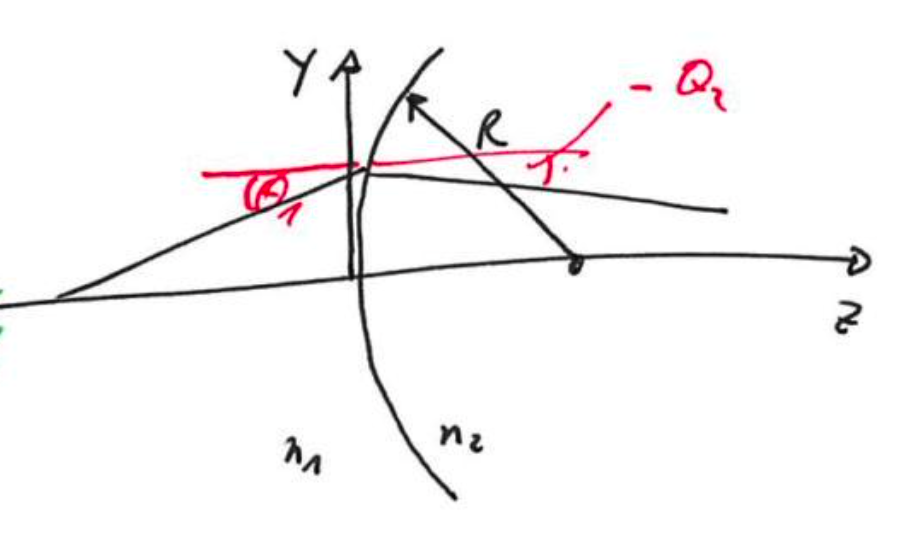
\includegraphics[width=\textwidth]{\currfiledir sketches/spherical_surface.png}
    \inputtikz{\currfiledir spherical_surface}
   \caption{Refraction of  a ray at a spherical surface}
\end{marginfigure}

We start with a ray of angle $\theta_1$ towards the optical axis in a medium of refractive index $n_1$. It hits the spherical surface at a height $y$ above the optical axis. Here we apply Snell's law and calculate the new direction of the ray. Using the paraxial approximation, we get
\begin{equation}
    \theta_2 \approx \frac{n_1}{n_2} \theta_1 =  \frac{n_2 - n_1}{n_2} \, \frac{y}{R} \quad .
    \label{eq:1_single_spherical_surface}
\end{equation}
Negative angles $\theta_i$ describe ray pointing towards below the optical axis.


We can do the same for many rays originating under different angles $\theta_1$ from  a point $P_1 =(y_1, z_1)$ in medium 1. We find that they all cross in a point $P_2 = (y_2, z_2)$ in medium 2. Point $P_1$ is thus imaged on point $P_2$. For convenience, the sign convention is thus that $z$ is measured from the intersection of the optical axis and the surface, i.e., both $z_i$ are positive.
We get
\begin{equation}
    \frac{n_1}{z_1} + \frac{n_2}{z_2} \approx \frac{n_2 - n_1}{R} \quad \text{and} \quad
    y_2 = - \frac{n_1}{n_2} \, \frac{z_2}{z_1} \, y_1 \quad .
\end{equation}
The position $z_2$ along the optical axis of the image point does not depend on $y_1$, i.e., every point in the plane $z=z_1$ will have its image in the plane $z = z_2$. These two planes are \emph{conjugate planes}.




\section{Thin lens}

We combine two spherical surfaces of radius $R_1$ and $R_2$. In the sketch \ref{fig:1_thin_lens} $R_2$ is negative, as this is a concave surface when seen along the optical axis. The two surfaces enclose a medium of refractive index $n$, while the outside is air, i.e., $n_1 = 1$.

\begin{marginfigure}
    %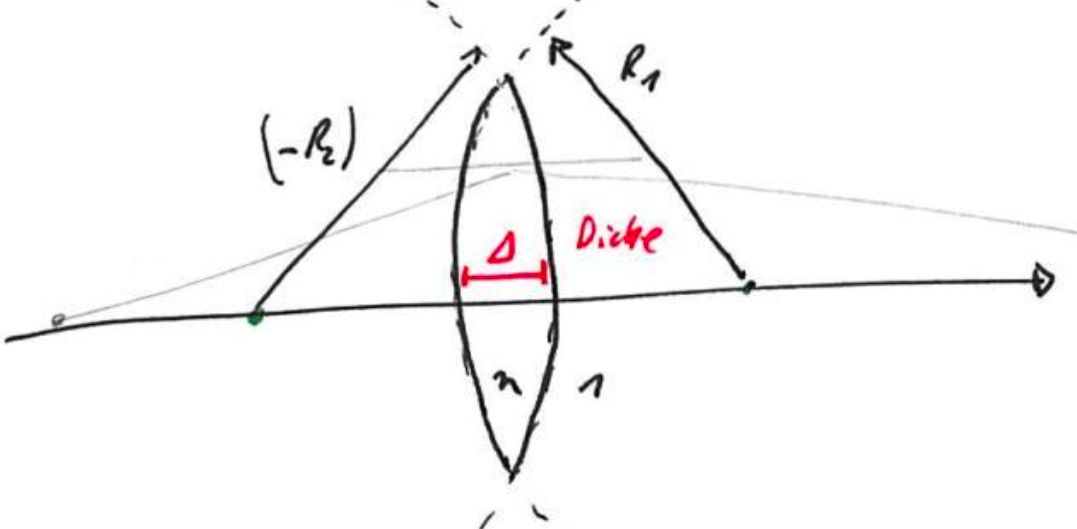
\includegraphics[width=\textwidth]{\currfiledir sketches/thin_lens.png}
    \inputtikz{\currfiledir lens}

   \caption{Refraction of  a ray at a thin lens}
   \label{fig:1_thin_lens}
\end{marginfigure}


We make the approximation that this is a \emph{thin lens}, i.e., that the width $\Delta$ of the lens on the optical axis is so small that we can neglect the change in height $y$ of the ray across the lens. We apply twice eq. \ref{eq:1_single_spherical_surface} and get
\begin{equation}
    \theta_2 = \theta_1 - \frac{y}{f} \quad \text{with} \quad
   \frac{1}{f} = (n-1) \left( \frac{1}{R_1} - \frac{1}{R_2} \right) 
\end{equation}
with the \emph{focal length} $f$. The coordinates of the image points are
\begin{equation}
    \frac{1}{z_1} + \frac{1}{z_2} = \frac{1}{f} \quad \text{and} \quad 
    y_2 = - \frac{z_2}{z_1} \, y_2 \quad .
\end{equation}
Again, this holds only in the paraxial approximation. When the rays make a too large angle with the optical axis, they will not be focused ideally. A spherical lens shows aberrations.

\begin{marginfigure}
    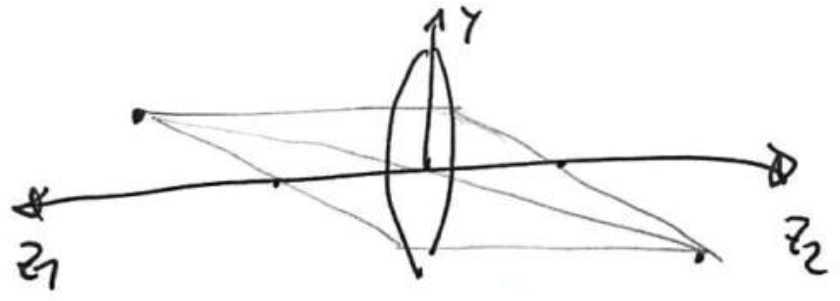
\includegraphics[width=\textwidth]{\currfiledir sketches/thin_lens_image.png}
   \caption{Image formation at a  thin lens}
   \label{fig:1_thin_lens_image}
\end{marginfigure}


For three special rays the action of a lens becomes very simple:
\begin{itemize}\setlength{\itemsep}{0pt}
    \item a ray that arrives parallel to the optical axis ($\theta_1 = 0$) will leave such that it passes through the focal point $(0,f)$ on the other side
    \item  a ray that arrives passing the  focal point will leave parallel to the optical axis
    \item a ray that passes through the center of the lens ($y = 0$) will remain unchanged
\end{itemize}
These rules have been formulated assuming a positive focal length $f$. When $f$ is negative, the same rules apply, but it  appears that the ray would have passed the  focal point on the other side of the lens. Additionally, it helps to remember that parallel rays will intersect in the focal plane.


\section{Matrix method}
When tracing a ray through an optical system, all you have to do is apply Snell's law at each interface. This is possible, but a bit tedious. A simpler approach is the idea of matrix optics. We describe a ray at a given position $z$ along the optical axis by two parameters: its angle $\theta$ with the optical axis and its height $y$ above the axis. We assume rotational symmetry so that $x=y$ and combine $\theta$ and $y$ into one vector. The effect of each optical element can then be written as a matrix acting on the vector, since in the paraxial approximation everything becomes linear.

\begin{marginfigure}
    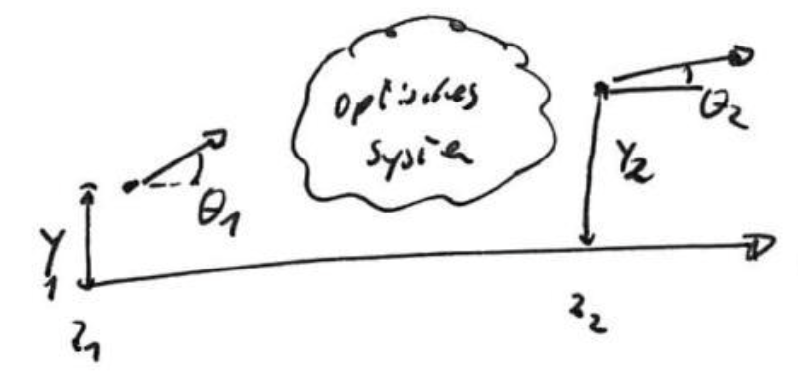
\includegraphics[width=\textwidth]{\currfiledir sketches/matrix_idea.png}
   \caption{The ray-transfer matrix describes the optical system between two planes.}
\end{marginfigure}

\paragraph*{Propagation} When a ray travels a distance $d$ through a homogeneous medium, its angle does not change. The height $y$ changes by $d \cdot \theta$. We write this as a ray-transfer matrix
\begin{equation}
    \begin{pmatrix}
        y_2 \\ \theta_2 
    \end{pmatrix}
    = 
    \boldsymbol{M}_\text{prop}
    \cdot
    \begin{pmatrix}
        y_1 \\ \theta_1 
    \end{pmatrix}
    \quad
    \text{with} \quad 
    \boldsymbol{M}_\text{prop} = 
    \begin{pmatrix}
        1 & d \\ 0 & 1
    \end{pmatrix} \quad .
\end{equation}

\paragraph*{Planar interface} Refraction at a planar interface does not change the height, but the angle
\begin{equation}
    \boldsymbol{M}_\text{planar} = 
    \begin{pmatrix}
        1 & 0 \\ 0 & \frac{ n_1 }{n_2}
    \end{pmatrix} \quad .
\end{equation}


\paragraph*{Spherical interface} Refraction at a spherical interface also does not change the height. The change in angle depends on ray height $y$
\begin{equation}
    \boldsymbol{M}_\text{spherical} = 
    \begin{pmatrix}
        1 & 0 \\ - \frac{n_2 - n_1}{n_2 R} &  \frac{ n_1 }{n_2}
    \end{pmatrix} \quad .
\end{equation}

\paragraph*{Thin lens} The action of a thin lens in paraxial apprixaltion is
\begin{equation}
    \boldsymbol{M}_\text{lens} = 
    \begin{pmatrix}
        1 & 0 \\ - \frac{1}{f} &  1
    \end{pmatrix} \quad .
\end{equation}


A sequence of optical elements is modelled as a product of ray transfer matrices. Note that the order is reversed. We typically propagate a ray from left to right, but mathematics is of Arabic origin, i.e. reads from right to left. The very first optical element is therefore represented by the rightmost matrix in the matrix product.

\section{Example: Point source in the focal plane of a lens }

As an example, let us calculate the effect of a point source that is placed in the focal plane of a thin lens. We start with a ray vector
\begin{equation}
\boldsymbol{v}_\text{in} = 
    \begin{pmatrix}
        y \\ \theta
    \end{pmatrix}  \quad , 
\end{equation}
let it propagate by a distance $d=f$ and then pass through a lens. In total we have
\begin{equation}
    \boldsymbol{v}_\text{out} = \boldsymbol{M}_\text{lens} \cdot  \boldsymbol{M}_\text{prop} \cdot \boldsymbol{v}_\text{in}
    = 
    \begin{pmatrix}
        y  + f \theta \\ - \frac{y}{f}
    \end{pmatrix} \quad .
\end{equation}
We see that the outgoing angle $\theta_\text{out} = - y/f$ does not depend on the direction $\theta$ in which the ray leaves the point source. All these rays are thus parallel, as expected.

\begin{marginfigure}
    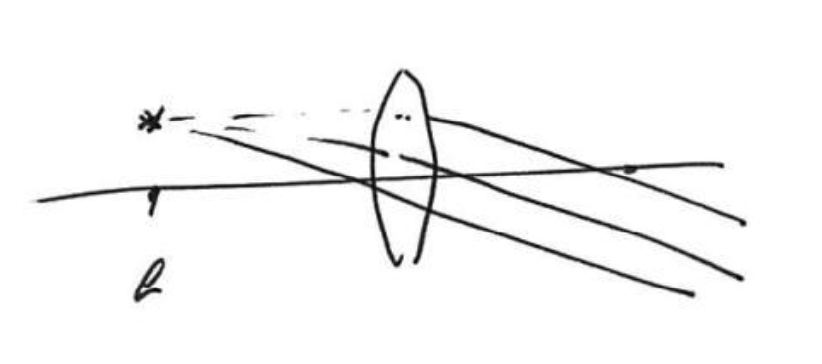
\includegraphics[width=\textwidth]{\currfiledir sketches/matrix_example.png}
   \caption{Point source in the focal plane of a lens }
\end{marginfigure}



\section{A thick lens with principal planes}

The approximation of a thin lens can be removed by introducing principal planes\sidenote{German: Hauptebenen}. It can be shown that the action of a thick lens (i.e, to spherical surfaces separated on the optical axis by a larger distance) and even the action of a sequence of lenses can be described as a single thin lens plus two principal planes. The rays enter the first principal plane and then immediately leave the second principal plane as if they would have passed an effective thin lens of focal length $f$. The position of the planes and the effective focal length are the only free parameters.


\begin{marginfigure}
    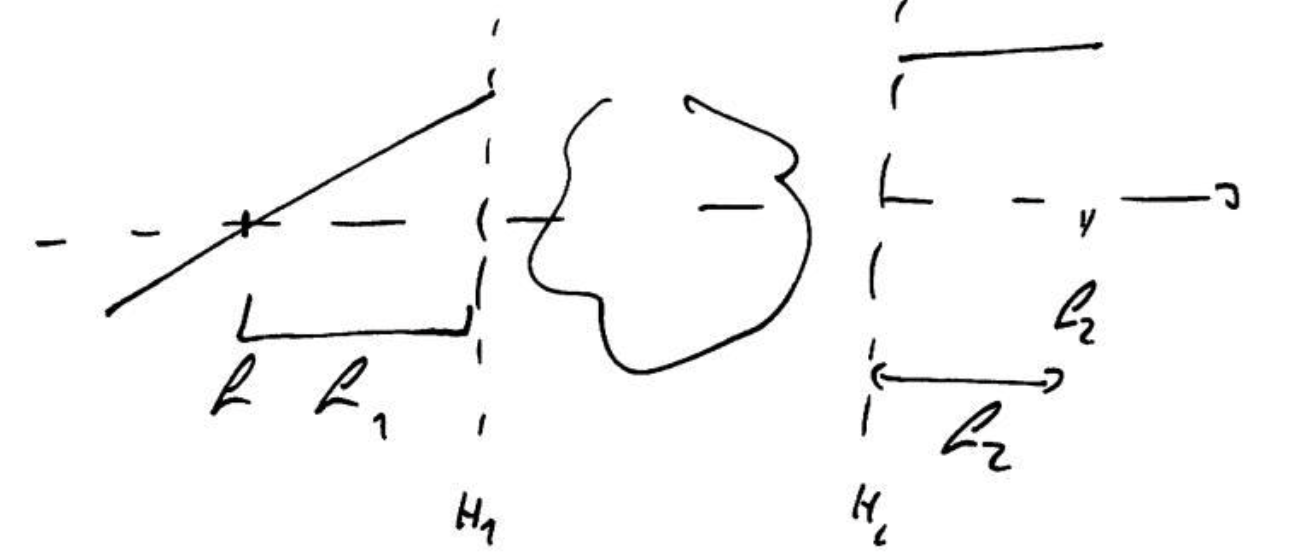
\includegraphics[width=\textwidth]{\currfiledir sketches/principal_plane.png}
   \caption{The two principal planes simplify many optical systems.}
\end{marginfigure}

\begin{questions}
\item A telephoto lens consists of many lenses, but can still be described by a single focal length. This focal length can be longer than the distance between the front lens and the film. The effective single lens is therefore outside the telephoto lens. This can be described by introducing principal planes in the matrix method of ray optics.
 
   Consider an optical element that can be described by a transfer matrix $\boldsymbol{M}$ with $\det(\boldsymbol{M}) = 1$. The two principal planes are located at distances $d_1$ before and $d_2$ after this element. These distances may also be negative. Assume that the refractive index of these domains is one. Show that these three domains together act like a thin lens and calculate $d_1$ and $d_2$.

\item  Show that any arrangement of thin lenses and distances between these lenses satisfies the above requirement $\det(\boldsymbol{M}) = 1$. \newline Hint: $\det(\boldsymbol{A} \boldsymbol{B} )  = \det(\boldsymbol{A})  \det(\boldsymbol{B}) $
\end{questions}


\section{Aberrations}
For\sidenote{This section is  adapted from \cite{Konijnenberg_Optics}} designing advanced optical systems Gaussian geometrical optics is not sufficient. 
Instead non-paraxial rays, and among them also non-meridional\sidenote{meridional rays run in a plane than contains the optical axis} rays, must be traced  using software based on Snell's Law with the sine of the angles of incidence and refraction. Often many thousands of rays are  traced to evaluate the quality of an image. 
It is then found that in general the non-paraxial rays do not intersect at the ideal Gaussian image point. Instead of a single spot, a spot diagram is found which is more or less confined. The deviation from an ideal point image  is quantified in terms of  \emph{aberrations}. One distinguishes between monochromatic and chromatic aberrations. The latter are caused by the fact that the refractive index depends on wavelength. The first are a consequence of the small angle approximation in paraxial optics. If instead one retains the first two terms of the Taylor series of the sine,  the errors in the image can be quantified by  five monochromatic aberrations, the so-called \emph{primary} or \emph{Seidel aberrations} (see, for example, wikipedia\sidenote{\url{https://en.wikipedia.org/wiki/Optical_aberration}}). The best known  is \emph{spherical aberration}, which is caused by the fact that for a convergent spherical lens, the rays that makes a large angle with the optical axis are focused closer to the lens than the paraxial rays (see Fig.~\ref{fig:1_Spherical_aberration}
). \emph{Distortion} causes deformation of images due to the fact that the magnification depends on the distance of the object point to the optical axis.



\begin{marginfigure}
  %  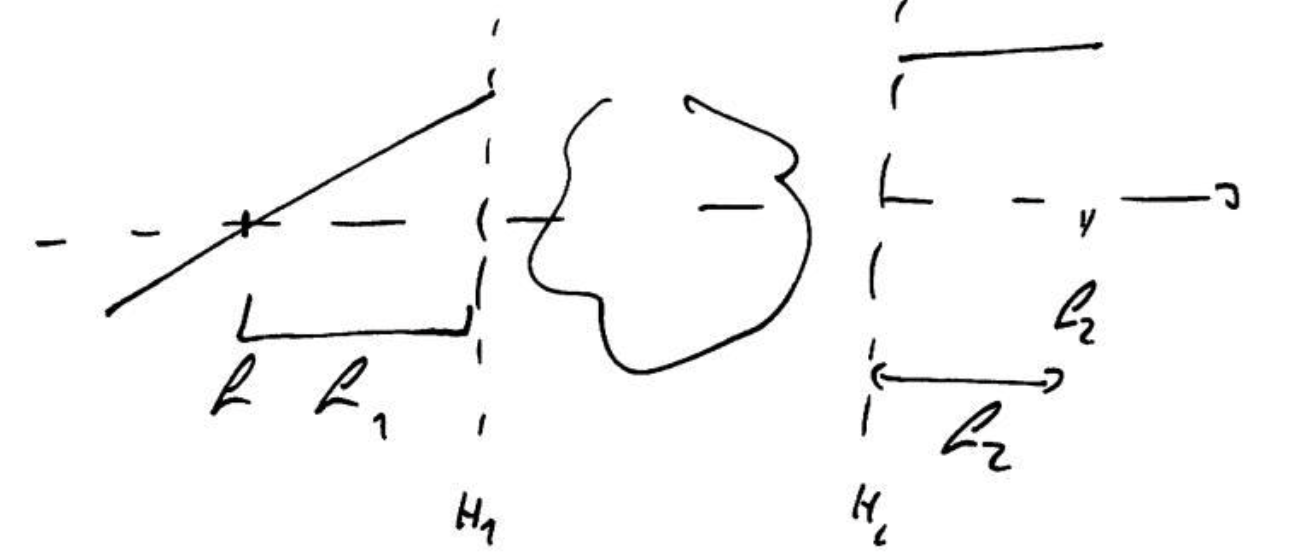
\includegraphics[width=\textwidth]{\currfiledir sketches/principal_plane.png}
   \caption{XXX spherical aberration}
\label{fig:1_Spherical_aberration}
\end{marginfigure}



For high-quality imaging the aberrations have to be reduced by adding more lenses and optimizing  the curvatures of the surfaces, the thicknesses of the lenses and  the distances between them. For high quality systems,  a lens with an aspherical surface is sometimes used.  Systems with very small aberrations are extremely expensive, in particular if the field of view is large, as is the case in  lithographic imaging systems used in the manufacturing of integrated circuits.




\section {Hands on: Aligning optical elements I}

In the practical part of this chapter, you should practice to align optical elements as mirrors, lenses and beam splitters.

\paragraph*{Laser beam} We will discuss in the next chapter the idea of a laser beam more iin detail. For now, it is sufficient to think of a bundle of rays that run more or less parallel to each other. So the beam is described by the diameter of the ray bundle and the angle of divergence within the bundle. Without lenses, we can for now assume that the rays remain parallel so that a laser beam can be approximated by a ray of geometrical optics.

\paragraph*{Degrees of freedom} It is useful to have in mind the degrees of freedom that a ray of light has. Above we have used $y$ and $\theta$ to describe a ray in a single plane. In three dimensions, we need two spatial coordinates $x$ and $y$, and two angles with the optical axis, say $\theta_x$ and $\theta_y$. If we want to align and thus define a beam, we need to fix these four degrees of freedom.

\paragraph*{Alignment tip} A three-dimensional volume above an optical table is quite huge. In almost all cases it is not needed. It is sufficient to restrict the beam to one plane parallel to the table surface. The height of the beam above the table is defined by tje alignment tip. The center of the tip should coincide with the center of the beam.

\paragraph*{Defining the first leg} The laser beam leaves the laser typically in an not too well defined direction and position. We then need two mirrors to define the four degrees of freedom of the beam as each mirror is described by two angles. We place the tip first after the second mirror and use the first mirror to bring the beam on the tip. Then we place the tip far from the second mirror and use the second mirror for alignment. Iterating this procedure will converge.\sidenote{The other way round does not converge!}

\paragraph*{Defining all further legs} The advantage of a fixed beam hight comes with all further legs of the beam path. At a third mirror, the beam has already the correct height. We place the mirror such that its surface sits at the intersection oif the first two legs. Then we use the two angles of the mirror to define the new direction of tge beam.

\paragraph*{Lenses} A lens should be centered on the beam. We first align the beam without lens, then place the tip after the intended position of the lens. We put the lens into the beam and translate perpendicular to the beam until it again goes over the tip. The angle of the lens relative to the beam can be check by back reflections. When translating the lens in beam direction, one needs to pay attention that the lens does not leave its centered position.

\paragraph*{Beam splitter} At a beam splitter, three rotational degrees of freedom come into play. The translational degrees are identical with those of a mirror.






%--------------------
\printbibliography[segment=\therefsegment,heading=subbibliography]

\renewcommand{\lastmod}{October 11, 2023}
\renewcommand{\chapterauthors}{Markus Lippitz}

\chapter{Gaussian Beams}


\goal{By the end of this chapter you should be able to explain the electric field in a Gaussian focus.
You can construct a Gaussian beam 'by hand' for typical lens systems and calculate it using the ABCD law.}


\section{Overview}

We extend our model to describe light. In this and the following chapters we will use wave optics and assume that light is a scalar wave. We will introduce typical wave functions as plane and spherical waves. Of particular importance are Gaussian beams: as eigenmodes of a laser resonator, they are ubiquitous in optical experiments. We will discuss how these waves and beams are transmitted through optical elements and how we can determine their properties.
More details on these topics can be found in chapter 2 and 3 of \cite{SalehTeich1991}, chapter 4.6 of \cite{Hering_Martin_Optik},  chapter 13 of \cite{Hecht_Optics}.



%-----------------------------------------------------------------------------
\section{Postulates of Wave Optics}

The wave function $u(\br, t)$ is complex-valued and fulfills the wave equation
\begin{equation}
    \nabla^2 u - \frac{1}{c^2} \, \frac{\partial^2 u}{\partial t^2} = 0
\end{equation}
with $c = c_0 /n$ the velocity of light in the medium of refractive index $n$. 
We do not yet assign a physical meaning to the wave function $u(\br, t)$. But since you have seen Maxwell's equations elsewhere, you might think of it as one component of the electric field, for example. At interfaces between media, the index of refraction $n$ changes and thus also $1/c$, but we still do not discuss the physics of such interfaces and partial reflection is beyond our scope.
The only connection we make to observable physical quantities is by defining the  \emph{intensity} $I$ of the wave as
\begin{equation}
    I(\br) = \braket{ |u(\br, t) |^2 }
\end{equation}
where the pointed brackets indicate a time average over a period long compared to the wave period.

A consequence of the linear wave equation is the superposition principle. If $u$ and $v$ are solutions to the wave equation, then also $\alpha u + \beta v$ is a solution. This also means that light beams cross themselves without interaction.


\section{Monochromatic waves}

The solutions of the wave equation can be written as harmonic functions
\begin{equation}
    u(\br, t)  = \tilde{u}(\br) \, e^{- i \omega t}
\end{equation}
with an angular frequency $\omega = 2 \pi \nu$. The spatial part $\tilde{u}(\br)$ fulfils the Helmholtz equation
\begin{equation}
    \nabla^2 \tilde{u} + k^2 \tilde{u} = 0 \quad \text{with} \quad k = \frac{\omega}{c} \quad .
\end{equation}
$k$ is called the \emph{wavenumber} and becomes the \emph{wavevector} when going to three dimensions. The intensity is then given by $\tilde{u}(\br)$
\begin{equation}
    I(\br) = \braket{ |u(\br, t) |^2 } = |\tilde{u}(\br) |^2 \quad , 
\end{equation}
i.e., the intensity of a monochromatic wave is constant in time. 

Lets discuss a few typical examples

\paragraph*{Plane wave} The amplitude $\tilde{u}$ is given by
\begin{equation}
 \tilde{u}(\br) = A \, e^{i \bk \cdot \br}
\end{equation}
with $\bk$ the wavevector and $|\bk| = k $. The \emph{wavefronts}, i.e., surfaces of constant phase $\phi = q \, 2 \pi =  \arg \tilde{u}(\br)$, are parallel and equidistant planes. The distance is the wavelength $\lambda = c / \nu = 2 \pi / k$.

When the index of refraction $n$ changes at an interface, the frequency $\omega$ remains the same, but the wavelength $\lambda$, the velocity of light $c$ and the wavenumber $k$ change
\begin{equation}
\lambda = \frac{\lambda_0}{n} \qquad
c = \frac{c_0}{n} \qquad
k = \frac{k_0}{n} \quad .
\end{equation}
 

\paragraph*{Spherical wave} Here the amplitude $\tilde{u}$ is given by
\begin{equation}
 \tilde{u}(\br) = \frac{A}{r} \, e^{i k r} \quad \text{with} \quad r = |\br| \quad .
 \label{eq:2_spherical_wave}
\end{equation}
Note that the right side of the equation does only use scalar variables. The wavefunction depends thus only on the distance to the origin and has spherical symmetry. The wavefronts are concentric spheres of distance $\lambda$.

\paragraph*{Paraboloidal wave} Close to the optical axis, we can approximate the spherical wave by a paraboloidal wave. We call $\theta$
\begin{equation}
    \theta^2 =  \frac{x^2 + y^2}{z^2} \ll 1
\end{equation}
and write $r$ as a Taylor expansion on $\theta$
\begin{align}
    r = & \sqrt{x^2 + y^2 + z^2}= z \sqrt{1 + \theta^2}
    = z \left( 1 + \frac{\theta^2}{2} - \frac{\theta^4}{8} + \cdots \right) \\
    \approx & z \left( 1 + \frac{\theta^2}{2} \right) = z + \frac{x^2 + y^2}{2z}  \quad .
\end{align}
This is called the \emph{Fresnel approximation}. We put it into eq.  \ref{eq:2_spherical_wave} and approximate in the amplitude term even $r \approx z$. We get
\begin{equation}
    \tilde{u}(\br) = \frac{A}{z} \, e^{i k z} \, e^{i k \, \frac{x^2 + y^2}{2z}  } \quad .
\end{equation}
For points close to the optical axis but far from the origin, a spherical wave approaches a planar wave. In between, the paraboloidal wave is a useful approximation.


\begin{marginfigure}
    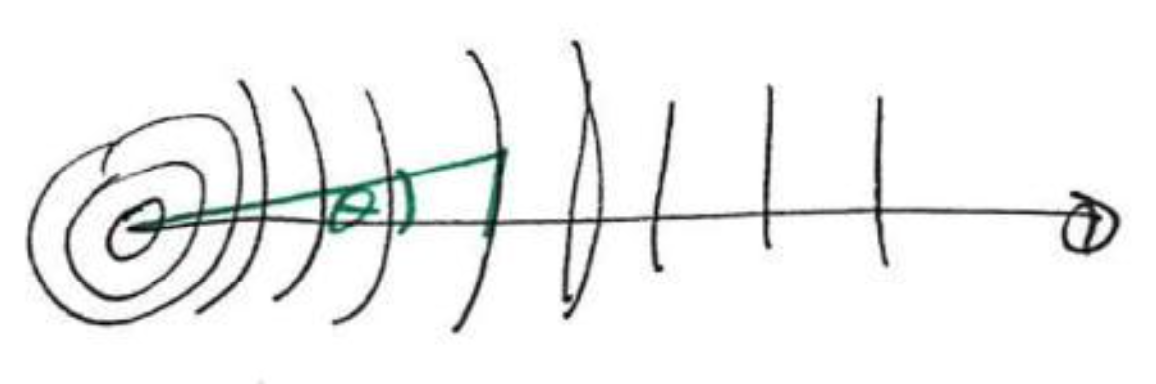
\includegraphics[width=\textwidth]{\currfiledir sketches/paraboloidal.png}
   \caption{XXX sketch Fig 2.2.4 S/T}
\end{marginfigure}


\section{A transparent plate}

As most simple optical element, we consider a transparent plate of thickness $d$ and index of refraction $n$ in air. We transmit a plane wave. The wavefunction is continuos at the interface. We are interested in the complex-valued transmission function $t(x,y)$
\begin{equation}
    t(x,y) = \frac{\tilde{u}(x,y,d)}{\tilde{u}(x,y,0)} \quad .
\end{equation}
For perpendicular incidence, the phase advances by $n k_0 d$ from left to right. The transmission function is thus
\begin{equation}
    t(x,y)  = e^{i n k_0 d} \quad .
\end{equation}

\begin{marginfigure}
    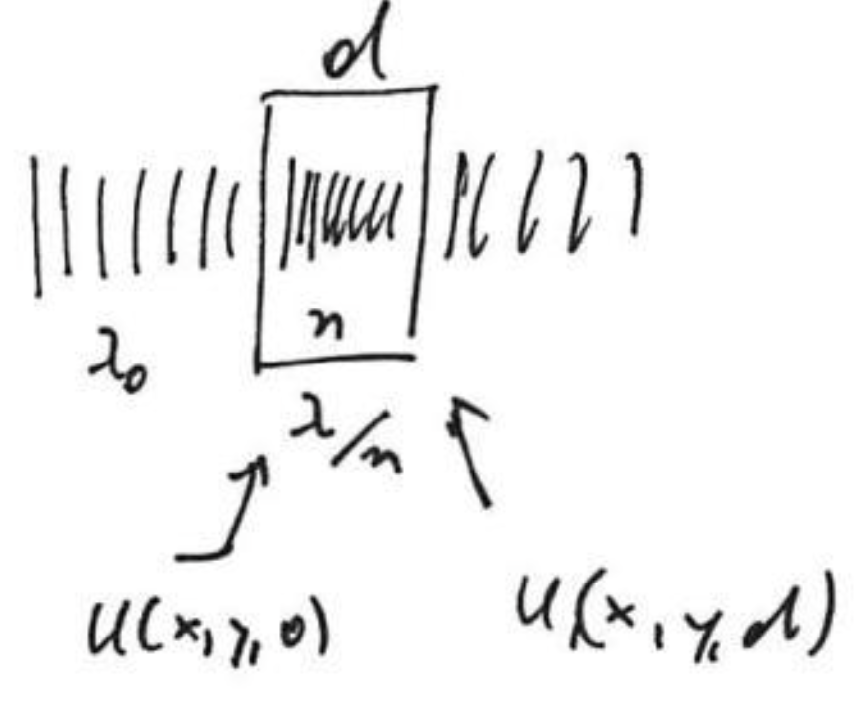
\includegraphics[width=\textwidth]{\currfiledir sketches/plate.png}
   \caption{A plate}
\end{marginfigure}


When the plane wave approaches the plate under angle $\theta$, then Snell's law gives the internal angle $\theta_i$ as $\sin \theta = n \sin \theta_i$. The wavevector makes this angle $\theta_i$ with the optical axis, so that the $z$-component of the term $\bk \cdot \br$ at the right side gives $n k \cos \theta_i$ and the total transmission function is
\begin{equation}
    t(x,y)  = e^{i n k_0 d \cos \theta_i} \quad .
\end{equation}
This is always against my intuition. The geometrical path in the plate gets longer by tilting it, but the phase difference becomes smaller. The point is that we only take the component along $z$ into account, as shifting a plane wave perpendicular to its direction of travel does not change anything.

We of course make again the approximation that the angle $\theta$ is small enough so that we can ignore the $\cos \theta_i$ part.

\begin{marginfigure}
    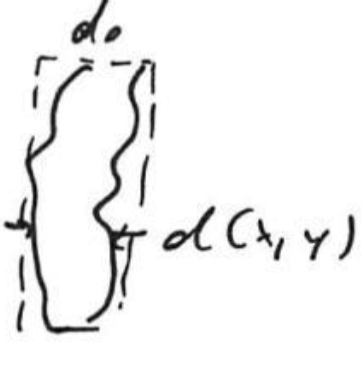
\includegraphics[width=0.5\textwidth]{\currfiledir sketches/plate_var_d.png}
   \caption{A plate of variable thickness}
\end{marginfigure}


If the plate has a variable thickness $d(x,y)$, we enclose it in a box of thickness $d_0$. Then part of the phase progression goes with $n$, part with air ($n=1$). In total this is
\begin{equation}
    t(x,y) \approx e^{i n k_0 d(x,y)} \,  e^{i k_0 (d_0 - d(x,y))}
    = h_0   e^{i (n-1) k_0 d(x,y)}
\end{equation}
with $h_0 = e^{i  k_0 d_0}$ a constant phase factor. This makes the approximation that all angles are small enough and neighboring parts of the plate do not 'mix' at the output.


\section{Conversion of a plane wave to a spherical wave by a lens}

\begin{marginfigure}
    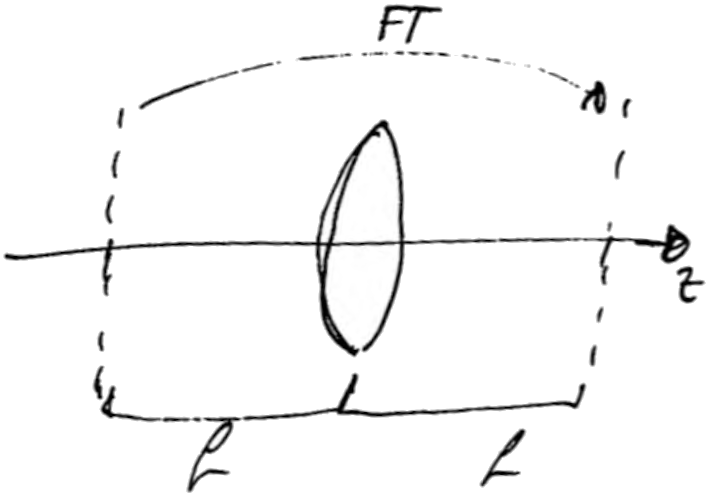
\includegraphics[width=\textwidth]{\currfiledir sketches/lens.png}
   \caption{A lens as plate of variable thickness}
\end{marginfigure}

The most interesting thin plate of variable thickness is a lens. For simplicity, we use a plane convex lens, i.e, set one radius of curvature to infinity. The thickness $d(x,y)$ of this plate is then
\begin{equation}
    d(x,y) = d_0 - \left( R - \sqrt{R^2 - (x^2 + y^2)} \right) \quad .
\end{equation}
We again use the Fresnel approximation $x^2 + y^2 \ll R^2$ and approximate the square-root term
\begin{equation}
    \sqrt{R^2 - (x^2 + y^2)}  = R \sqrt{1- \frac{x^2 + y^2}{R^2}} 
    \approx R \left( 1 -  \frac{x^2 + y^2}{2 R^2} \right)
\end{equation}
so that 
\begin{equation}
    d(x,y) \approx d_0 -  \frac{x^2 + y^2}{2 R^2} \quad .
\end{equation}
The transmission function is then
\begin{equation}
    t(x,y)= h_0 \,  e^{-i k_0 \frac{x^2 + y^2}{2f}}
    \quad 
    \text{with} \quad
    f = \frac{R}{n-1}
    \label{eq:2_phase_of_lens}
\end{equation}
and $h_0 = e^{i n k_0 d_0}$ another constant phase factor that we ignore.

A spherical lens thus transforms a plane wave into a paraboloidal wave centered around $z=f$.


\section{Gaussian beams as a paraxial solution of the wave equation}

When we have discussed typical solutions to the wave equation above, we started from the full wave equation, found spherical waves as solution, and then made the paraxial approximation to arrive at the paraboloidal waves. We could also have gone a different route. We can apply the paraxial approximation to the wave equation directly. This leads to the paraxial Helmholtz equation
\begin{equation}
    \nabla_T^2 A + i 2k \frac{\partial A}{\partial z} = 0
    \quad 
    \text{and}
    \quad
    \tilde{u}(\br) = A(\br) \, e^{i k z}
\end{equation}
with $ \nabla_T$ acting only on the transverse coordinates only. The envelop $ A(\br)$ modulates the carrier $\exp(i k z)$. $A$ needs to be \emph{slowly varying}, i.e., on a wavelength length scale it should not change much.

The paraboloidal waves 
\begin{equation}
    \tilde{u}(\br) = \frac{A}{z} \, e^{i k z} \, e^{i k \, \frac{x^2 + y^2}{2z}  }
\end{equation}
i.e.,
\begin{equation}
    A(\br) = \frac{A_1}{z}  \, e^{i k \, \frac{x^2 + y^2}{2z}  }
\end{equation}
fulfil this paraxial Helmholtz equation. The interesting point is that we can come to other solutions of the paraxial Helmholtz equation by replacing $z$ by $q(z) = z - i z_0$, i.e.
\begin{equation}
    A(\br) = \frac{A_1}{q(z)}  \, e^{i k \, \frac{x^2 + y^2}{2q(z)}  } \quad .
\end{equation}
These are \emph{Gaussian beams}. We call $q$ the q-parameter and $z_0$ the \emph{Rayleigh range}. We separate the complex function $1/q(z)$ into its real and imaginary part
\begin{equation}
    \frac{1}{q(z)} = \frac{1}{z -i z_0} = \frac{1}{R(z)} + i \frac{\lambda}{\pi W^2(z)} \quad .
\end{equation}
We will see that $R$ and $W$ give the wavefront radius of curvature and the beam width, respectively. Putting everything together, the wavefunction reads
\begin{equation}
    \tilde{u}(\br) = A_0 \, \frac{W_0}{W(z)} \, 
    \exp \left( - \frac{\rho^2}{W^2(z)}  \right) \, 
    \exp \left( +i kz +ik  \frac{\rho^2}{2 R(z)}  - i \zeta(z) \right) 
\end{equation}
with
\begin{align}
    W(z) = & W_0 \sqrt{1 + \left( \frac{z}{z_0} \right)^2    } \label{eq:2_wz} \\
    R(z) = & z \left[ 1 + \left( \frac{z_0}{z} \right)^2 \right] \\
    \zeta(z) = & \arctan \frac{z}{z_0} \\
    W_0 = & \sqrt{\frac{\lambda z_0}{\pi}} \quad . \label{eq:2_w0}
\end{align}
Note that there are only two independent parameters next to the wavelength $\lambda$, namely the amplitude $A_0$ and the Rayleigh range $z_0$.



\section{Parameters and Properties of Gaussian Beams}

Let us discuss some properties of a Gaussian beam. The \emph{intensity} $I$ is
\begin{equation}
    I(\rho, z) = | \tilde{u}(\rho, z) |^2 = I_0 \left( \frac{W_0}{W(z)}  \right)^2 \, e^{- \frac{2 \rho^2}{W(z)^2} }
\end{equation}
i.e, the transversal profile of the intensity is a Gaussian. Along the $z$ axis
\begin{equation}
    I(0, z) =  I_0 \left( \frac{W_0}{W(z)} \right)^2= \frac{I_0}{1 + \left( \frac{z}{z_0} \right)^2}  \approx I_0  \left( \frac{z_0}{z} \right)^2
\end{equation}
where we assumed $z \ll z_0$ in the last approximation. This means that the intensity drops as $1/z^2$, as a spherical wave.

At the \emph{beam waist} ($z=0$), the width $W(z=0) = W_0$ describes the radial distance $\rho$ at which the intensity  has dropped to $1/e^2$ of the peak value. When moving one Rayleigh range $z_0$ out of the focus, this radius increases by $\sqrt{2}$, as $W(z_0) = \sqrt{2} W_0$. At this distance, the intensity on the axis has dropped by a factor $1/2$. When integrating over any surface perpendicular to the optical axis, the integrated intensity or power remains the same.

\begin{marginfigure}
    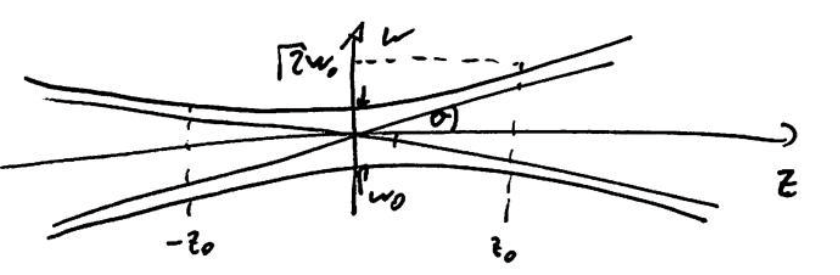
\includegraphics[width=\textwidth]{\currfiledir sketches/gauss_divergence.png}
   \caption{Divergence of a Gaussian beam}
\end{marginfigure}


We can define a \emph{divergence}, or opening angle $\Theta$ of the Gaussian beam. Far away from the beam waist, i.e. $z \ll z_0$ we have
\begin{equation}
    W(z) \approx W_0 \frac{z}{z_0} = \Theta \, z \quad \text{with} \quad \Theta = \frac{W_0}{z_0} = \frac{\lambda}{\pi W_0} \quad .
 \end{equation}
 Note that next to the wavelength $\lambda$ only the Rayleigh range $z_0$ \emph{or} the beam waist $W_0$ is a free parameter, not both. The divergence of the beam is fully contained in the beam waist. One can interpret this as diffraction of the Gaussian beam at its own waist. For comparison, diffraction at a circular aperture of radius $R$ would  lead to an angle $\Theta_\text{app} = 0.61 \lambda  / R$.

 \begin{figure}
    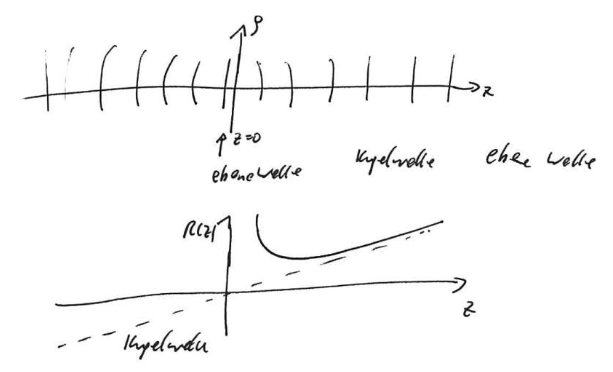
\includegraphics[width=\textwidth]{\currfiledir sketches/gauss_phase.png}
   \caption{Phase fronts and radius of curvature $R$ around the beam waist.}
\end{figure}

The phase of the Gaussian beam is given by the imaginary factors of the exponential function, i.e.
\begin{equation}
    \phi(\rho, z) = k z + k  \frac{\rho^2}{2 R(z)}  -  \zeta(z) 
\end{equation}
and the curvature of the phase fronts by 
\begin{equation}
    R(z) = z \left[ 1 + \left( \frac{z_0}{z} \right)^2 \right]  \quad .
\end{equation}
At the focus ($z=0$) and for $z \rightarrow \infty$ we find a diverging radius of curvature, i.e., a plane wave. For large distances this is the same as for a circular wave. Around the focus, the Gaussian beam differs as the radius of curvature changes such that we also get a plane wave exactly at $z=0$. Another peculairity of Gaussian beams is the \emph{Gouy phase} $\zeta(z)$
\begin{equation}
    \zeta(z) =  \arctan \frac{z}{z_0}  \quad .
\end{equation}
When passing through the focus, the wave undergoes a $pi$ phase shift. An intuitive picture could be the following\footcite{Boyd1980IntuitiveEO}: In geometrical optics, the ray would go through the focus. In a Gaussian beam, the path along the $1/e$ contour stays on the same side of the optical axis and in thus around the focus a bit shorter. This is compensated by the Gouy phase shift.


%XXX M Parameter ??


\section{Gaussian beams as eigenmodes of a resonator}
The importance of Gaussian beams comes from the laser as a ubiquitous light source. A laser produces Gaussian beams because these wave functions are the eigenmodes of a resonator formed by two spherical mirrors.

In a laser, we are interested in eigenmodes, i.e. optical wave functions that do not change as they bounce back and forth in the resonator. The mirrors in a laser cavity are typically so highly reflective that there are many round trips before the field leaves the cavity.


\begin{marginfigure}
    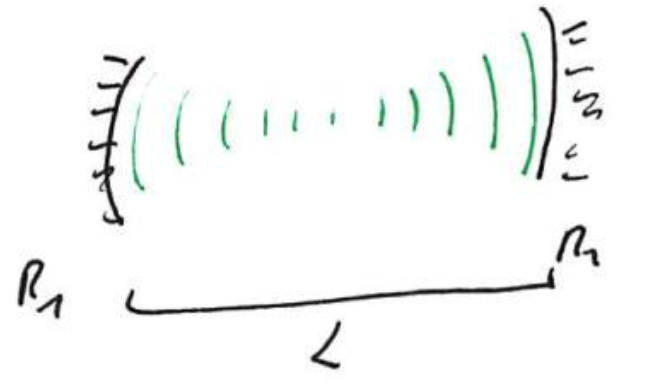
\includegraphics[width=\textwidth]{\currfiledir sketches/cavity.png}
   \caption{Eigenmodes of a laser cavity}
\end{marginfigure}


For an eigenmode to occur, the wavefront of the mode at the position of the mirror must match the shape of the mirror, otherwise it will reflect back into itself. The design of the cavity gives the radius of curvature $R_1$ and $R_2$ and the distance $d$ between the mirrors. We now show that under certain conditions a Gaussian beam is an eigenmode of such a cavity.

We search for the positions $z_1$ and $z_2$ of the mirrors and the Rayleigh range $z_0$ if the mean. We have the equation system
\begin{align}
    z_2 = & z_1 + d \\
    R_1 = & z_1 \left[ 1 + \left( \frac{z_0}{z_1} \right)^2 \right] \\
    R_2 = & z_2 \left[ 1 + \left( \frac{z_0}{z_2} \right)^2 \right]  \quad .
\end{align}

The solution is
\begin{align}
    z_1 = & \frac{-d (R_2 + d)}{R_1 + R_2 + 2d} \\
    z_2 = &z_1 + d  \\
    z_0^2 = & \frac{-d (R_1 +d)(R_2 + d)(R_1 + R_2 +d)}{(R_1 + R_2 + 2d)^2} \quad .
\end{align}
For a Gaussian beam $z_0$ must be real (or $z_0^2 > 0$). Otherwise $q = z - i z_0$ would be real and we would get a paraboloidal wave. This results in the \emph{stability condition} of a spherical cavity
\begin{equation}
    0 \le \left( 1 + \frac{d}{R_1} \right) \left( 1 + \frac{d}{R_2} \right) \le 1
\end{equation}

XXX sketch of stability condition

\section{Thin lens}

What happens when a Gaussian beam passes through a thin lens? We assume a thin lens, so $z$ does not change. The radial amplitude distribution $ \tilde{u}(\rho, z)$ also does not change, which means that the width parameter $W$ remains the same, i.e,
\begin{equation}
    W^{(L)} = W^{(R)} \quad .
\end{equation}
The phase needs a bit more attention. Just before the lens, the phase of the Gaussian beam is
\begin{equation}
   \phi^{(L)} =  k z + k  \frac{\rho^2}{2 R}  -  \zeta(z) 
\end{equation}
The phase effect of a lens is (see eq.~\ref{eq:2_phase_of_lens})
\begin{equation}
  \Delta\phi_\text{lens} =   - k \frac{\rho^2}{2f}
\end{equation}
so that after the lens we have in total
\begin{equation}
  \phi^{(R)} =  \phi^{(L)}   + \Delta\phi_\text{lens}  =   k z   -  \zeta(z)  + k  \left( \frac{\rho^2}{2 R} - \frac{\rho^2}{2f} \right)
\end{equation}  
i.e. 
\begin{equation}
    \frac{1}{R^{(R)}} = \frac{1}{R^{(L)}} - \frac{1}{f} \quad .
\end{equation}

What does this mean for the other properties of a Gaussian beam? How are Rayleigh range $z_0$ and beam waits $W_0$ modified by a lens? Knowing $\lambda$, $W(z)$ and $R$, i.e, the beam properties at the lens, we can use eqs.~\ref{eq:2_wz}--\ref{eq:2_w0}  to calculate $z_0$, $W_0$ and $z$, i.e. the focal parameter and the distance $z$ of focus and lens. We get
\begin{align}
    W_0 = & \frac{W(z)}{\sqrt{1 + \left(\frac{\pi W(z)}{ \lambda R(z)} \right)^2}} \\
    z = & \frac{R(z)}{1 + \left(\frac{\pi W(z)}{ \lambda R(z)} \right)^2} \quad .
\end{align}
We thus can connect the left and right beam parameters.



\begin{figure}
    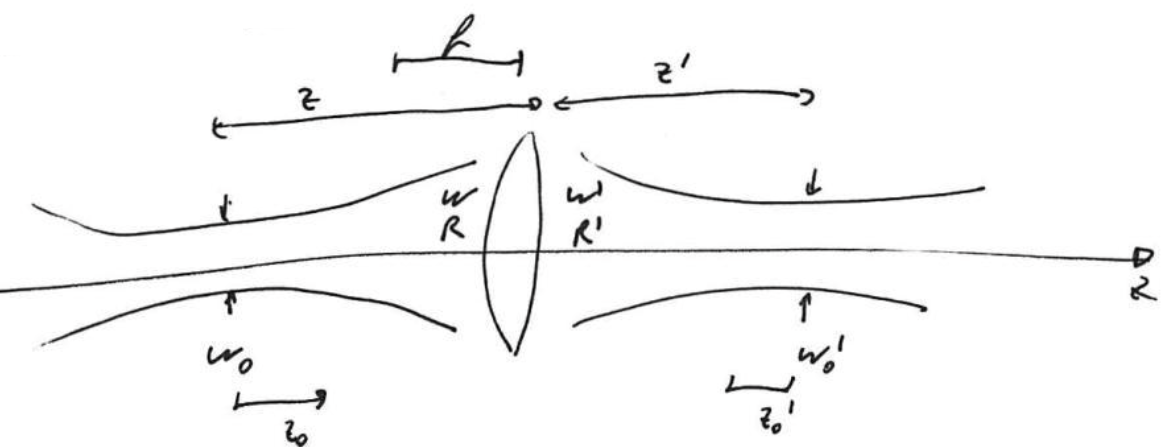
\includegraphics[width=\textwidth]{\currfiledir sketches/gauss_lens.png}
   \caption{A lens acting on a Gaussian beam}
\end{figure}


When the left beam waist is far from the lens, then we can see this arrangement as imaging of the left beam waist to a position $z^{(R)}$ on the right side  of the lens, which will magnify the beam waist radius. The magnification factor in ray optics is 
\begin{equation}
    M_r = \left| \frac{f}{z^{(L)} -f}  \right| \quad \text{and} \quad W_0^{(R)} \approx M_r W_0^{(L)}  \quad .
\end{equation}
The requirement 'far enough' means $z^{(L)} - f \gg z_0^{(L)} $, or
\begin{equation}
    r = \frac{z_0^{(L)} }{z^{(L)}  - f} \ll 1 \quad .
\end{equation}
We can calculate the beam parameters without  this approximation using a general magnification factor $M$ and obtain
\begin{align}
    M = & \frac{M_r}{\sqrt{1 + r^2}} \\
    W_0^{(R)}  = & M W_0^{(L)}  \\
    (z^{(R)} - f) = &M^2 (z^{(L)} -f) \\
    z_0^{(R)} = & M^2 z_0^{(L)}  \\
    \Theta_0^{(R)} = & \frac{\Theta_0^{(L)} }{M} \quad .
\end{align}

\section{ABCD Law and q parameter}

Things become simpler when we realize that the $q$ parameter is governing the Gaussian beam. We introduced above the Gaussian beams by 
\begin{equation}
    q(z) = z - i z_0 \quad \text{and} \quad
    \frac{1}{q(z)} = \frac{1}{R(z)} + i \frac{\lambda}{\pi W^2(z)} \quad .
\end{equation} 
As soon as we know $q$ at a single position along the beam, we can calculate all the rest. When $q_1$  and $q_2$ describe the $q$ parameters left and right of an optical element, both are connected by the \emph{ABCD law}
\begin{equation}
    q_2 = \frac{A q_1 + B}{C q_1 + D}
\end{equation}
where 
\begin{equation}
\boldsymbol{M} = 
\begin{pmatrix}
    A & B \\ C & D \\
\end{pmatrix}
\end{equation}
is the $2\times2$ matrix of the matrix method in ray optics, as introduced in the last chapter.\sidenote{see \cite{Brooker_Optics}, chapter 7.9, for a justification.}

\emph{Propagation} by a distance $d$ thus leads to 
\begin{equation}
    q_2 = q_1 + d \quad .
\end{equation}
The action of a \emph{lens} is described by
\begin{equation}
    q_2 = \frac{f q_1}{f - q_1} \quad .
\end{equation}


%\section{Bonus: Hermit- and Laguerre-Gaussian beams}


\section{Technique: Knife Edge Test}


A common tool for determining the properties of a Gaussian beam is a knife edge or razor blade. We mount it so that it can be moved perpendicular to the optical axis, cutting out a variable part of the beam. If we measure the power in the beam after the knife edge as a function of its position, we get a partial integral over the cross-section of the beam.
\begin{equation}
    P(x_0) = \int_{x=x_0}^\infty \int_{y=-\infty}^\infty I(x,y) \, dx \, dy \quad .
\end{equation}
Taking the numerical derivative yields the beams intensity profile.
\begin{equation}
    I(x) \propto \frac{\partial P(x_0)}{\partial x_0} \quad .
\end{equation}


We can also observe the shadow of the knife edge to determine the position of the beam waist. We place a screen far from the waist and the knife edge at the estimated waist position. If the knife is between the waist and the screen, the shadow will start from the same side as the knife enters the beam. If the knife is further away than the waist, the directions are reversed. If the knife is exactly at the waist, the image on the screen will turn dark with no apparent direction. This is the \emph{Foucault knife edge test} to determine the position and quality of a focus, originally of a spherical mirror.

\begin{questions}
    \item Explain why the image turns dark with no apparent direction.
\end{questions}

%--------------------
\printbibliography[segment=\therefsegment,heading=subbibliography]


\part{Fourier optics}
\renewcommand{\lastmod}{September 26, 2023}
\renewcommand{\chapterauthors}{Markus Lippitz}

\chapter{Fourier Optics}

\goal{By the end of this chapter you should be able to explain and experimentally demonstrate the filtering of spatial frequencies.}




\section{Overview}
Fourier transformation simplifies the description of light, especially when it passes through obstacles, as in diffraction. The action of a lens also involves a Fourier transform. This is the field of \emph{Fourier optics}. I will follow chapter 4 of \cite{SalehTeich1991} here. Another good source is \cite{Goodman2005}. Note that books (as Saleh \& Teich) from the engineering  side of optics use $j = - i = - \sqrt{-1}$ instead of $i$. Sometimes this $j$ is even written as $i$, so engineering is the complex conjugate of physics.


We will briefly lay the foundations of Fourier optics and then discuss diffraction and optical Fourier transform through a lens. For our purposes it is sufficient to consider scalar waves, i.e. we ignore the vectorial nature of the electric (or magnetic) field of light and use only a complex scalar value at each point in space to describe light. We will need fundamental properties of the Fourier transformation, as de scribed in Appendix \ref{chap:appendix_Fourier}
. For numerical applications Appendix \ref{chap:appendix_FFT}
might be useful.

\section{Spatial frequencies}

Let us start with a plane wave
\begin{equation}
    U(\br) = A e^{i \bk \cdot \br} \quad \text{with} \quad k = | \bk | = \frac{2\pi}{\lambda} \quad .
\end{equation}
We assume that all three components of $\bk$ are real (\emph{far-field optics} in contrast to \emph{near-field optics}), but the amplitude $A$ might be complex.
The wave vector $\bk$ makes the angles $\Theta_{x,y}$ with the $x$--$z$ and the $y$--$z$ plane, respectively, with
\begin{equation}
    \sin \Theta_x = \frac{k_x}{k} \quad .
\end{equation}
In the $z=0$ plane, the field is
\begin{equation}
  U(x,y,0) = f(x,y) = A \, e^{2 \pi \, i (\nu_x x + \nu_y y) }
\end{equation}
with the \emph{spatial frequencies} $\nu_x$ and $\nu_y$ 
\begin{equation}
  \nu_{x,y} = \frac{k_{x,y}}{2 \pi} = \frac{1}{\Lambda_{x,y}}
\end{equation}
and the period of the field $\Lambda_{x,y}$ in the $x$ and $y$ direction. And of course all this is related, i.e.,
\begin{equation}
    \sin \Theta_x = \frac{k_x}{k} = \lambda \nu_x = \frac{\lambda}{\Lambda_x}
\end{equation}
and similar for the $y$ direction. The assumption of all-real $\bk$ components makes sure that for all combinations of $k_x$,$k_y$, $k_z$ an angle $\Theta$ can be found, i.e., the right side of the equation is real and below one in absolute value. 

We will almost always make the \emph{paraxial approximation} assuming that the wave vector is roughly parallel to the $z$-direction, the angles $\Theta_{x,y}$ are thus small, and $k_{x,y} \ll k$. Then we can omit the sine in the last equation and get 
\begin{equation}
     \Theta_x \approx \frac{k_x}{k} = \lambda \nu_x = \frac{\lambda}{\Lambda_x} \quad .
\end{equation}

What happened here? The combination of all-real $\bk$ components, i.e., optical far-field, and fixed wavelength $\lambda$ removes one degree of freedom in the three components of the wave vector. As long as we know the wavelength and we know that the plane wave is nicely propagating, only two  real values are enough to fully describe it. These two values could be the angles $\Theta_{x,y}$, or the spatial frequencies $\nu_{x,y}$ or the $\Lambda_{x,y}$.


\section{Transmittance function}

A plane wave of amplitude one is traveling in $+z$ direction. At $z=0$ it is transmitted through a thin optical element with the complex  transmittance function $f(x,y)$ with
\begin{equation}
    f(x,y) =  e^{2 \pi \, i (\nu_x x + \nu_y y) } \quad .
\end{equation}
Directly after this plate, the optical field is $U(x,y,0) = f(x,y)$, i.e., the field is modulated by the transmittance function. We know from above that such a field is traveling in the direction given by the $\Theta_{x,y}$ or equally by the spatial frequencies $\nu_{x,y}$. The field is thus diffracted in this direction.\sidenote{This is not an optical grating yet, as this would change the amplitudes only, i.e., have a real-valued tranmittance function.}

In general, if the transmittance function $f$ would have an arbitrary shape, it could be decomposed into a sum of harmonic functions. Each harmonic component would diffract a part of the plane wave into its direction. So when we express $f$ by its Fourier transform $F$
\begin{equation}
    f(x,y) = \mathcal{FT} \left\{ F(\nu_x, \nu_y) \right\}
     = \iint F(\nu_x, \nu_y)  \, e^{2 \pi \, i (\nu_x x + \nu_y y) } \, d\nu_x  d\nu_y
\end{equation}
then we get
\begin{equation}
    U(x,y,0) 
     = \iint F(\nu_x, \nu_y)  \, e^{2 \pi \, i (\nu_x x + \nu_y y) } \, d\nu_x  d\nu_y \quad .
\end{equation}
This becomes useful when calculating the field \emph{at any point in space}, i.e., by including the $z$ coordinate:
\begin{equation}
    U(x,y,z) 
     = \iint F(\nu_x, \nu_y)  \, e^{2 \pi \, i (\nu_x x + \nu_y y) } \,e^{i k_z z} \, d\nu_x  d\nu_y \quad ,
     \label{eq:2_Uxyz}
\end{equation}
where $k_z$ now depends on the integrating variables
\begin{equation}
    k_z = \sqrt{k^2 - k_x^2 - k_y^2} = 2 \pi \left( \frac{1}{\lambda^2} - \nu_x^2 - \nu_y^2 \right) \quad .
    \label{eq:2_Uxyz_kz}
\end{equation}
Again the requirement of propagating waves entails $\nu_x^2 + \nu_y^2 <  1/\lambda^2$, so not all Fourier components of $F$ play a role.


\section{Transfer function and impulse response}

Let us first introduce the concepts with electric  circuits such as an RC-filter. One can define a transfer function $H(\omega)$ that relates the frequency spectrum $F(\omega)$ at the input (of the filter) with that at the output 
\begin{equation}
    G(\omega) = F(\omega) \cdot H(\omega) \quad .
\end{equation}
In time domain, the impulse response $h(t)$ is another description. The signal $f(t)$ at the input results in an output $g(t)$
\begin{equation}
    g(t) = \int h(\tau) f(t - \tau) d\tau \quad ,
\end{equation}
where causality requires that $h(t)$ is zero for $t <0$. The interesting point is that not only the signals $f$ and $g$ are connected to their Fourier transforms $F$ and $G$, but also the transfer function $H$ is the Fourier transform of the impulse response $h$. A Fourier transform converts a product into a convolution, and vice versa.


\section{Transfer function of free space}

We now apply this scheme to spatial frequencies describing a superposition of plane waves. Letting the wave propagate by a distance $d$ from a source plane $f(x,y) = U(x,y,0)$ to a target plane $g(x,y) = U(x,y,d)$, how do the spatial amplitudes $F$ and $G$ relate? Looking at eq.  \ref{eq:2_Uxyz}, we see that it is just the last exponential function  that depends on $z$, but we need to take eq.  \ref{eq:2_Uxyz_kz} into account. Together we find
\begin{equation}
    H(\nu_x, \nu_y) = \exp \left(  
  2 \pi \, i  \, d \, \sqrt{ \frac{1}{\lambda^2} - \nu_x^2 - \nu_y^2 }
    \right) \quad .
\end{equation}
For spatial frequencies $\nu_x^2 + \nu_y^2 <  1/\lambda^2$, i.e., within a circle of radius $1/\lambda$, the magnitude does not change ($|H| = 1$), only the phase changes. Outside this circle, the magnitude drops exponentially width $d$, as the square-root becomes imaginary. These waves are called \emph{evanescent waves}, as they do not propagate and only exist in the near-field.

High spatial frequencies $\nu$ near $1/\lambda$ are far away from the paraxial approximation. In most cases it is sufficient to restrict ourself to low spatial frequencies $ \ll 1/\lambda$. In this case, we can use the \emph{Fresnel approximation} of the transfer function
\begin{equation}
    H(\nu_x, \nu_y)_\text{Fresnel} = H_0 \exp \left(  
   - 2 \pi \, i  \, d \, (
 \nu_x^2 + \nu_y^2 )
    \right) \quad \text{with} \quad H_0 = e^{i k d} \quad .
\end{equation}
The term $H_0$ factors out the trivial phase evolution due to propagation along the optical axis.

When we know the spatial frequency amplitudes $F$ at $z=0$, then we obtain $G$ at $z=d$ by
\begin{equation}
    G(\nu_x, \nu_y) =  F(\nu_x, \nu_y) \cdot  H(\nu_x, \nu_y) \quad .
\end{equation}
We can Fourier transform the equation to obtain 
\begin{equation}
    g(x,y) = f(x,y) \otimes h(x,y) \label{eq:2_gfh_conv}
\end{equation}
where $\otimes$ signals a convolution. The impulse response of free space is in the Fresnel approximation
\begin{equation}
    h(x,y)_\text{Fresnel} \approx h_0 \, \exp \left(i k \frac{x^2 + y^2 }{2d} \right) \quad \text{with} \quad
    h_0 = -\frac{i}{\lambda d} \,  e^{i k d } \quad .
\end{equation}
Eq. \ref{eq:2_gfh_conv} means that we get from one plane to the other by convolving each source point with a wave of shape $h$. This is equivalent to the Huygens principle, where each point should be a source of a spherical wave. When we take the paraxial approximation of a spherical wave we obtain $ h(x,y)_\text{Fresnel}$.


\section{Optical Fourier transform by propagation}

Up to now we used the Fourier transform to simplify description of optical fields. In this section, we will show that the propagation of an optical field by a long enough distance allows to optically 'compute' the Fourier transform. We will find that the field in the target plane $g(x,y)$ is proportional to the Fourier transform $F$ of the field in the source plane.

\begin{marginfigure}
    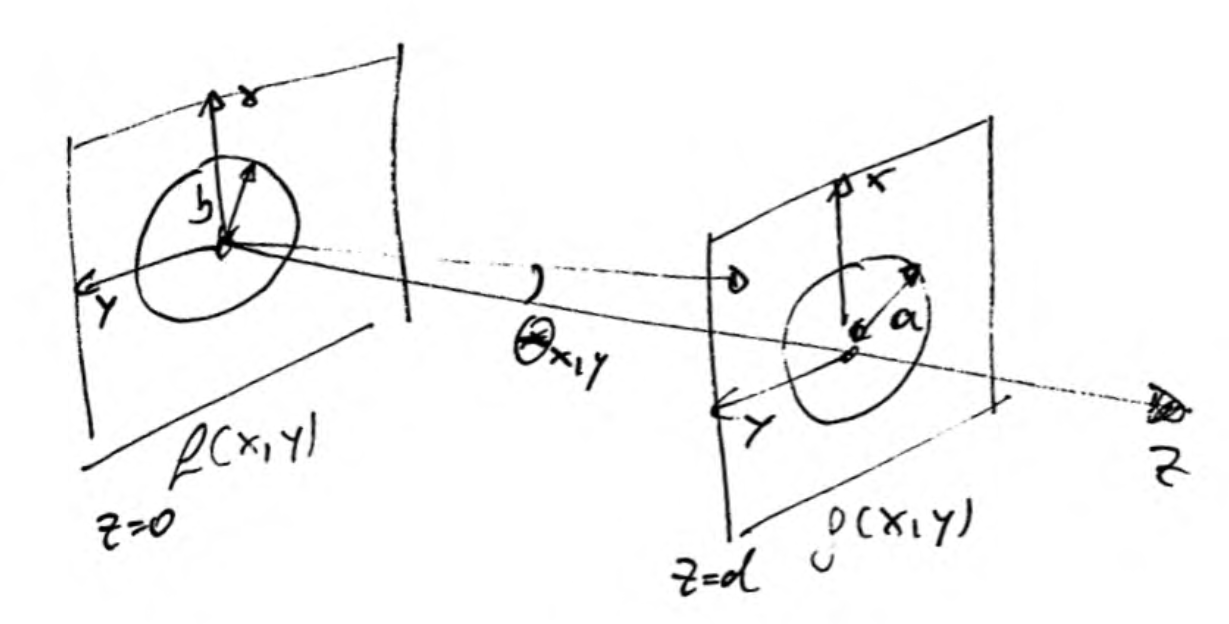
\includegraphics[width=\textwidth]{\currfiledir sketches/fraunhofer.png}
    \caption{Fraunhofer condition}
\end{marginfigure}

The Fourier components $F$ of the field $f$ in the source plane determine the direction of travel of the plane waves, as we have seen above. The problem is that a plane wave is everywhere in space. We need thus to find a condition for 'far enough' so that the individual pieces of the plane wave have separated enough. We do not only employ the paraxial approximation, i.e., that the wave vectors are not too inclined on the optical axis. The key point is that we also require the size of the source plane to be limited. This leads to the two conditions of the Fraunhofer approximation
\begin{equation}
    N_F =  \frac{a^2}{\lambda d} \ll 1 \quad \text{and} \quad
    N_{F}' =  \frac{b^2}{\lambda d} \ll 1 
\end{equation}
where the two $N_F$ are the Fresnel numbers, and $a$,$b$ are the radius of the relevant and allowed regions in the target and source planes, respectively. $d$ is again the distance between the  planes. The Fraunhofer approximation is a more severe restriction than the Fresnel approximation.

We start by writing down the convolution integral of eq. \ref{eq:2_gfh_conv} in the Fresnel approximation
\begin{align}
    g(x,y) = & f(x,y) \otimes h(x,y)_\text{Fresnel} \\
 = & h_0 \iint f(x', y') \,  \exp \left(i k \frac{(x-x')^2 + (y-y')^2 }{2d} \right)  \, dx' dy' \quad .
\end{align}
The term $(x-x')^2$ in the exponent of the exponential function is multiplied out into three terms. 
We keep the mixed terms. Both squared terms can be neglected due to the Fraunhofer approximation. For example  we get 
\begin{equation}
    \exp \left(i \pi  \frac{x'^2 + y'^2 }{ \lambda d} \right) \approx 1
\end{equation}
as  $N_{F}' \ll 1$. The terms without prime vanish due to $N_{F} \ll 1$. So we have
\begin{equation}
    g(x,y)  \approx h_0   
     \iint f(x', y') \,  \exp \left(-i 2 \pi \frac{x x' + y y' }{\lambda d} \right)  \, dx' dy' \quad .
\end{equation}
We now identify  the factor $x / \lambda d$ with the spatial frequency  $\nu_x$ ($y$ similar) and write
\begin{equation}
    g(x,y) \approx h_0
     F \left( \nu_x,\nu_y \right) 
     =  h_0
     F \left( \frac{x}{\lambda d}, \frac{y}{\lambda d} \right) \quad .
\end{equation}

When we place a screen $g$ at a distance fulfilling the Fraunhofer condition after a diffracting obstacle $f$, the interference pattern visible on the screen will be described by the Fourier transform $F$ of $f$. This simplifies a lot the calculation of single slit, double slit and grating, as typically  presented in the  introductory optics lecture.

\begin{questions}
    \item Convince yourself that the textbook solution, for example in Demtröder, can be obtained by a Fourier transform.
    \item Estimate the required distance so that a typical diffraction grating fulfils the Fraunhofer condition.
\end{questions}


\section{Optical Fourier transform by a lens}

The distance $d$ required to stay within the Fraunhofer approximation can be prohibitively large. We will see here that a lens is able to shorten the distance between the grating and the screen and still keep the Fourier relation. This explains why spectrometers are not too long, but contain a lens or curved mirror.

\begin{marginfigure}
    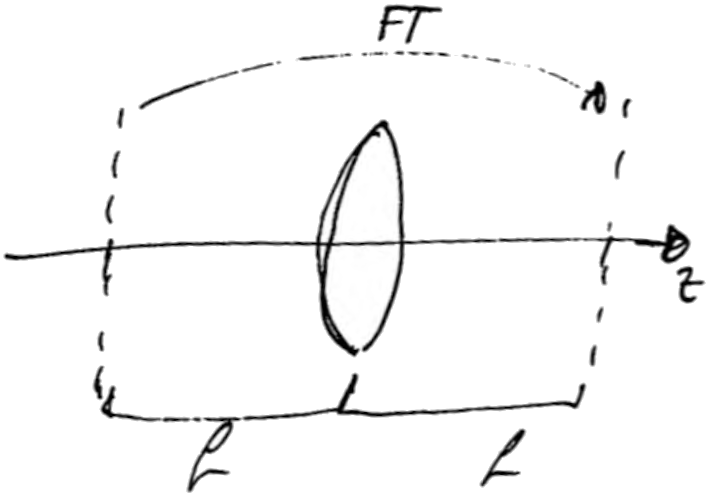
\includegraphics[width=\textwidth]{\currfiledir sketches/lens.png}
    \caption{Optical Fourier transform by a lens}
\end{marginfigure}

From geometrical optics in the paraxial approximation we know already that a lens focuses a beam  (angles $\Theta_x$, $\Theta_y$ to the optical axis) on a point 
\begin{equation}
(x,y) = (f \Theta_x, f \Theta_y)
\end{equation}
in the focal plane, where $f$ describes the focal length of the lens. A lens thus separates plane waves by their propagation direction. As in the beginning of the chapter, we can convert angles into optical frequencies and thus find that the field in the target plane $g$ is proportional the the Fourier amplitude $F$
\begin{equation}
    g(x,y) = \tilde{h} \,   F \left( \nu_x,\nu_y \right) = \tilde{h} \,  F \left( \frac{x}{\lambda d}, \frac{y}{\lambda d} \right) \quad .
\end{equation}
The remaining question is the prefactor $\tilde{h}$. If it would depend of the spatial coordinates $x$ and $y$, this would destroy the Fourier transform. To obtain $\tilde{h}$, we multiply the transfer functions of free space for the distance source plane to lens (length $d$) and lens to target plane (length $f$). And we need to multiply a transfer function for the lens, as the lens has a thickness profile $t(x,y)$ of a material with a certain index of refraction. All together one obtains\sidenote{details in \cite{SalehTeich1991}, chapter 4}
\begin{equation}
    \tilde{h}(x,y) =  \tilde{h}_0 \exp \left( 
-i \pi \frac{(x^2 - y^2)(d-f)}{\lambda^2 f}
    \right) \quad \text{with} \quad  \tilde{h}_0  = \frac{-i}{\lambda f} \, e^{ik (d+f)} \quad .
\end{equation}
This factor becomes spatially constant when the condition $d=f$ is met. A lens thus performs an optical Fourier transform between is two focal planes. In a spectrometer, the grating sits in the front focal plane of the curved mirror (acting as a lens), the detector in its back focal plane.




\section{Spatial filter}


In addition to spectrometers, the spatial filter is another important application of a lens as a Fourier transform device. We consider a so-called 4f-system, see \cite{SalehTeich1991}. All components are separated by one focal length $f$: a source plane $f$, a first lens, a filter plane $p$, a second lens and a target plane $g$. Both lenses are identical. 

\begin{marginfigure}
    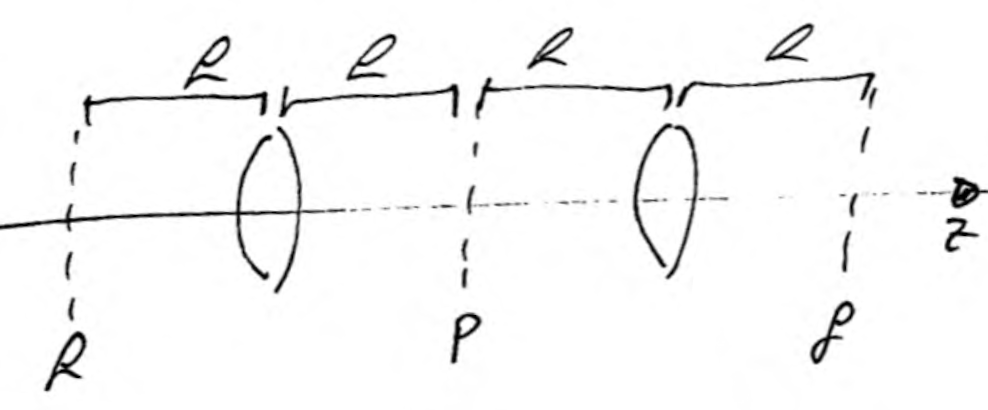
\includegraphics[width=\textwidth]{\currfiledir sketches/spatial_filter.png}
    \caption{A $4f$ system can be used as spatial filter.}
\end{marginfigure}

Let the transfer function $p$ of the filter plane be $p(x,y)=1$ for the beginning. Then the first lens Fourier transforms $f$ into $F$ in the filter plane. The filter does nothing and the second lens transforms back $F$ into $f$, so that we get in the target plane what we started with , i.e., $f=g$. Of course this make the assumption that all plane waves nicely propagate, i.e., the spatial frequencies in $f$ are small enough to cause only propagating plane waves.

The filter plane can be used to modify the Fourier components $F$. At position $x$ in the $p$ plane, only the Fourier component $\nu_x = x / (\lambda f)$ is present. We can put a mask $p(x,y)$, either just absorbing or with a complex transfer function in the filter plane. The overall transfer function of the 4f-system is then
\begin{equation}
    H(\nu_x, \nu_y) = p (\lambda f \nu_x, \lambda f \nu_y) \quad , 
\end{equation}
ignoring an overall phase factor for the propagation. 

An often used transfer function is a circular aperture. It removes all spatial frequencies above a certain threshold. In this way, one can clean up a laser beam, so that is follows the expected Gaussian profile even after transmission though many non-ideal optical elements.

The inverse filter, i.e. a opaque disc, acts as high-pass filter, increasing the edges in an optical image. A vertical slit lets only pass horizontal features in the image.



\section{Resolution of a microscope}

\section {Optical data processing: Correlation by Fourier transform }

\cite{Goodman2005}, chap. 8


%-----------------------------------------------------------------------------
\section{Hands on: Align  a pin hole}

Alignment strategy. Optimum diameter


%--------------------
\printbibliography[segment=\therefsegment,heading=subbibliography]


\part{Light in matter}
\renewcommand{\lastmod}{November 24, 2023}
\renewcommand{\chapterauthors}{Markus Lippitz}

\chapter{Dielectric Materials}

\goal{By the end of this chapter you should be able to explain and experimentally demonstrate total internal reflection and the Brewster effect.}



\section{Overview}

With this chapter we begin to consider the optical properties of media beyond their refractive index. The physics of the medium will play a role and have consequences for the propagation of light. To be able to do this, we also have to describe light as an electromagnetic wave, with three components for the electric and magnetic field, and not only as a scalar wave as in the last chapters. This will lead to the phenomenon of absorption and dispersion. We will also be able to assign a value to the amplitude of the reflected and transmitted waves at an interface.  These topics are described in chapter 5 and 6 of \cite{SalehTeich1991} and chapter 3 of \cite{Hecht_Optics}.


\section{Maxwells equations}

For completeness, let us start with the Maxwell equations in their macroscopic form
\begin{align}
\nabla \, \bD = & \rho \\
\nabla \, \bB = & 0 \\
\nabla \times \bE =  & - \dot{\bB} \\
\nabla \times \bH = & \dot{\bD} + \bj \quad .
\end{align} 
Matter comes in by the respective material equations
\begin{align}
    \bD = & \epsilon_0 \bE +  \bP = \epsilon \epsilon_0 \bE \\
    \bH = & \frac{1}{\mu_0} \bB - \bM =   \frac{1}{\mu \mu_0} \bB \\
    \bj = & \sigma \bE \quad .
\end{align}
Note that I use a unit-free dielectric function $\epsilon$. In literature, one finds different other methods to write the term $\epsilon \epsilon_0$. At the second equal sign we have assumed in each case a linear and isotropic medium. Let us define these and similar terms:
%
\begin{description}
    \item[linear] The relation between the electric field $\bE(\br, t)$ and the polarization $\bP(\br, t)$ is linear.
    \item[isotropic] The relation between $\bE$ and $\bP$ is independent of the direction of $\bE$. This also means that $\bE$ and $\bP$ are parallel.
    \item[homogeneous] The relation between $\bE$ and $\bP$ is independent of the position $\br$.
    \item[nondispersive] The relation between $\bE$ and $\bP$ is instantaneous, i.e., it depends only on the value of $\bE$ at time $t$, but not on earlier times. As we will see, this is equivalent to saying that the relation does not depend on the frequency $\omega$ of light. This is a thought model and is only approximated by real materials.
    \item[local] The relation between $\bE$ and $\bP$ depends only on the value of $\bE$ at one point $\br$, not at other points. This is also called \emph{spatially nondispersive}. Optical active media (next chapter) are nonlocal.
\end{description}


\section{Wave equations}
When we assume a source-free medium ($\bj = 0$, $\rho = 0$), one can derive the wave equation for an isotropic  and linear medium
\begin{equation}
    \nabla^2 \, \bE = \frac{n^2}{c_0^2} \ddot{\bE} \quad \text{with} \quad c_0^2 = \frac{1}{\mu_0 \epsilon_0} \quad ; \quad   n^2 = \epsilon \quad; \quad  \mu \approx 1 
\end{equation}
A similar equation exists for $\bH$. The individual vector components of the electrical and magnetic field fulfil thus the scalar wave equation of chapter \ref{chap:2_gauss}.

The flow of electromagnetic energy is described by the Poynting vector\sidenote{John Henry Poynting, 1852--1914}
\begin{equation}
    \bS = \bE \times \bH
\end{equation}
The intensity $I$ of a wave on a surface with normal $\boldsymbol{n}$ is the temporal average of the Poynting vector, i.e.
\begin{equation}
    I = \braket{\bS \cdot \boldsymbol{n}}_T = \frac{c \, n \, \epsilon_0}{2} \, | \bE_0 |^2 = \frac{1}{2 \eta } \, | \bE_0 |^2
\end{equation}
where $\bE_0 $ is the amplitude of the electrical field and $\eta = \sqrt{ \mu \mu_0 / (\epsilon \epsilon_0)}$ the impedance of the medium. For vacuum, $\eta_0 \approx$~\SI{377}{\ohm} . An intensity of 10~W/cm$^2$ corresponds to an electric field of about 87~V/m.

The Poynting vector fulfills the Poynting theorem: the flow of energy through a surface enclosing a volume either changes the energy density within that volume or performs work on magnetic or electric dipoles. As equation:
\begin{equation}
    \nabla \bS = - \frac{\partial}{\partial t} \left( \frac{1}{2}  \epsilon \epsilon_0 \bE^2 + \frac{1}{2} \mu \mu_0 \bH^2  \right)
    + \bE \cdot \frac{\partial \bP}{\partial t} +   \mu_0 \bH \cdot \frac{\partial \bM}{\partial t}
\end{equation}


As with scalar waves, we find different solutions to the wave equation. The plain wave also exists as electromagnetic wave:
\begin{align}
    \bH(\br, t) = & \bH_0 \, e^{i (\bk \br - \omega t)} \\
    \bE(\br, t) = & \bE_0 \, e^{i (\bk \br - \omega t)} 
\end{align}
with $|\bk| = k = 2 \pi n / \lambda_0$ and $\bH_0$, $\bB_0$ and $\bk$  orthogonal on each other. The electromagnetic wave is thus a \emph{transversal} wave.

The vectorial electromagnetic forms of paraboloidal wave and Gaussian beams can be constructed by vectorizing the scalar waves $u(\br)$ of the preceding chapters:
\begin{equation}
    \bE(\br) = \mathcal{E}_0 \left( - \hat{\bx} + \frac{x}{z + i z_0} \hat{\bz} \right) u(\br)
\end{equation}
where $\hat{\bx}$ and $\hat{\by}$ are unit vectors pointing in x and z direction, respectively, and $\mathcal{E}_0 $ is a scalar amplitude. $z_0$ is set to zero for a paraboloidal wave.

\section{Phenomenological approach to absorption}

Let us begin by describing absorption in media without attributing a microscopic origin. The susceptibility $\chi$ is complex-valued
%\sidenote{note the minus in front of the $i$!}
, i.e. $\chi = \chi' + i \chi''$ and thus the dielectric function 
\begin{equation}
    \epsilon = 1 + \chi = 1 + \chi' + i \chi'' = \epsilon' + i \epsilon''
\end{equation}
This means that the wave number $k$ will become complex, too
\begin{equation}
    k = \frac{\omega}{c} =  k_0 \sqrt{\epsilon} = k_0 \sqrt{1 + \chi' + i \chi''} = \beta + i \frac{\alpha}{2}
\end{equation}
The meaning of the real-valued $\alpha$ and $\beta$ will become clear when we use this definition in a plane wave:
\begin{equation}
    \mathcal{E}(z,t) =  \mathcal{E}_0 \,  e^{ i (k z - \omega t)} =
     \mathcal{E}_0 \, e^{-i \omega t} \, e^{i \beta z} \, e^{- \alpha z / 2}
\end{equation}
The intensity of this waves thus drops as
\begin{equation}
    I(z) \propto |\mathcal{E}(z,t) |^2 = |\mathcal{E}_0|^2 \, e^{- \alpha z}
\end{equation}
$\alpha$ is thus the absorption coefficient\sidenote{or attenuation or extinction coefficient}. Positive $\alpha$ means a decay of intensity, negative $\alpha$ would mean a gain, as in a laser. $\beta$ describes the progression of the phase or wave fronts. It is related to the real part $n$ of the refractive index\sidenote{I use the form $\tilde{n}= n + i \kappa$.} by $\beta = n k_0$. Everything together we have
\begin{equation}
    n + i \kappa = \frac{\beta}{k_0} + i \, \frac{1}{2} \, \frac{\alpha}{k_0} = \pm \sqrt{1 + \chi' + i \chi''}
    \label{eq:4_n_chi}
\end{equation}
The sign of the square root is chosen such that a  positive (absorbing) $\chi''$ leads to a positive (absorbing) $\alpha$, independent of the sign of $\chi'$. As we will see below $\chi' < 0$ is possible, e.g., near resonances.

It is convenient to have approximate forms of eq.  \ref{eq:4_n_chi} for the limiting cases of weak and strong absorption
\begin{align}
    \chi'' \ll 1 + \chi' &  \rightarrow& n \approx \sqrt{1 + \chi'} && \alpha \approx  \frac{k_0}{n} \chi'' \\
    \chi'' \gg |1 + \chi'| & \rightarrow & n \approx \sqrt{\chi'' / 2} && \alpha \approx 2 k_0 \sqrt{ \chi'' / 2}
\end{align}



\section{The Kramers-Kronig relations}

So far, we have only discussed the relationship between the applied external field $E(t)$ and the resulting polarization $P(t)$ for 'monochromatic' fields of the type $\exp(-i \omega t)$, i.e. for a precisely defined frequency $\omega$:
\begin{equation}
P(t) = \chi(\omega) \epsilon_0 E(t) \quad \text{for} \quad E(t) = E_0 e^{-i \omega t} \quad .
\end{equation}
This gave the frequency dependence of $\chi(\omega)$. We can generalize this for any time evolution of the field $E(t)$. The susceptibility is the \emph{impulse response} of the material, the memory so to speak:
\begin{equation}
P(t) = \epsilon_0 \int_{-\infty}^{+\infty} \chi( \Delta t = t - t') \, E(t') \, dt' \quad \text{for} \quad E(t) = \text{any} \quad .
\end{equation}
The polarization $P$ now, i.e. at time $t$, depends on the electric field at all other times $t'$. How strong the fields are depends only on the time interval $\Delta t$. Causality requires that the polarization 'now' does not depend on the field amplitudes in the future. Therefore $\chi( \Delta t = t - t' < 0) $ must be zero. This means that the susceptibility $\chi( \Delta t ) $ is complex, but known over half of the time ray as fixed to zero. This has consequences for the Fourier transform, i.e. for $\chi(\omega)$.

These consequences can be derived with the help of function theory\sidenote{see also Appendix A of \cite{Yariv1989}} and are the Kramers-Kronig relations. The following relationship exists between the real ($\chi'$) and imaginary ($\chi''$) parts of the susceptibility if they obey causality:
\begin{align}
 \chi'(\nu) = & \frac{2}{\pi} \, P \int_0^\infty \frac{s \, \chi''(s)}{s^2 - \nu^2} \, ds \\
 \chi''(\nu) = & \frac{2}{\pi}\, P \int_0^\infty \frac{\nu \, \chi'(s)}{\nu^2 - s^2} \, ds \quad .
 \label{eq:diel_KK}
\end{align}
$P$ denotes the Cauchy principal value integral. Similar relationships also exist for $\chi(\omega)$ and $\epsilon(\omega)$ as well as for all other variables that are subject to causality.

In principle, it is therefore sufficient to measure the real part of the susceptibility $\chi(\omega)$ in order to determine the imaginary part and thus the complete complex-valued function. Unfortunately, however, the integrals in Eq~\ref{eq:diel_KK} run over the entire frequency range from zero to infinity, which is of course not accessible experimentally. The Kramers-Kronig relations can still be used sensibly by making appropriate assumptions about the course outside the measured interval.



\section{Lorentz oscillator model}

The response of matter to an electric field is governed by the charged ions and electrons. Restoring forces lead to resonances depending on the frequency of the optical field. In the infrared, bound ions resonate, while in the ultraviolet, bound electrons dominate.


\begin{marginfigure}
\inputtikz{\currfiledir lorentz_oscillator}

\caption{Frequency dependence of the real and imaginary parts of the Lorentz oscillator. The real and imaginary parts of the complex-valued refractive index $\tilde{n}$ look qualitatively the same. \label{fig:diel_lorentz}}
\end{marginfigure}

The Lorentz oscillator model is a simple model that can be used to describe the frequency dependence of the dielectric function in the vicinity of resonances. In a damped harmonic oscillator (mass $m$, damping constant $\gamma$, natural frequency $\omega_0$), the mass is deflected by a periodic electric field (amplitude $E_0$, frequency $\omega$) by $x$ because the mass carries a charge $e$. All together
\begin{equation}
 m \ddot{x} + \gamma \dot{x} + m \omega_0^2 x = e E_0 e^{- i \omega t} \quad .
\end{equation}
The stationary solution of this differential equation is
\begin{equation}
 x(t) = \frac{e \, E_0}{m (\omega_0^2 - \omega^2) - i \gamma \omega} \, e^{- i \omega t} \quad .
\end{equation}
The macroscopic polarization $P$ is the sum of all microscopic polarizations, i.e.
\begin{equation}
P(t) = N \, e \,x(t) = (\epsilon -1 ) \epsilon_0 \, E_0 e^{- i \omega t}
= \chi \epsilon_0 E(t) \quad .
\end{equation}
This results in the dielectric function
\begin{equation}
\epsilon(\omega) = 1 + N \alpha = 1 +\frac{N e^2}{\epsilon_0} \frac{1}{m (\omega_0^2 - \omega^2) - i \gamma \omega} = \epsilon' + i \epsilon'' \quad .
\end{equation}
Explicit real and imaginary parts are
\begin{align}
 \epsilon' = & 1 + \frac{N e^2}{\epsilon_0} \frac{ m (\omega_0^2 - \omega^2)}{m^2 (\omega_0^2 - \omega^2)^2 + \gamma^2 \omega^2}  \\
  \epsilon'' = & \frac{N e^2}{\epsilon_0} \frac{ \gamma \omega }{m^2 (\omega_0^2 - \omega^2)^2 + \gamma^2 \omega^2}  \quad .
\end{align}


\begin{questions} 
\item Analogous to Figure \ref{fig:diel_lorentz}, show the frequency dependence of the components of the refractive index, i.e. of $n$ and $k$.

\item Approximate the real and imaginary parts of $\epsilon$ near resonance at $\omega_0$ as a function of $\Delta \omega = \omega - \omega_0$. In the case of the real part, only the range $| \Delta \omega | \gg \gamma/m$ is of interest.
\end{questions}




\section{Normal and  anomalous dispersion}

The visible spectral region is at a higher frequency than the resonance of the bound ions in the infrared, but at a lower frequency than that of the bound electrons in the ultraviolet. The real part $n$ of the refractive index   increases  with frequency, i.e. $n(\text{blue}) > n(\text{red})$ (see Fig. \ref{fig:diel_lorentz}). This is called 'normal' dispersion. It causes red light to deviate less than blue light in a prism and to be focused by a lens at a greater distance. On the energetically 'other' side of a resonance, the opposite behavior can be observed, 'anomalous dispersion'.
\begin{marginfigure}
    \inputtikz{\currfiledir multiple_lorentz_oscillator}
\caption{The visible spectral range lies between two resonances. \label{fig:diel_lorentz}}
\end{marginfigure}


The Lorentz-shaped resonance can be shown in a demonstration experiment. The imaginary part of the dielectric function Fig.~\ref{fig:diel_lorentz} determines the absorption and thus the line shape in the absorption spectrum of atoms or molecules. The real part determines the dispersion, i.e. the refractive index of a medium. A simple method of determining the refractive index is to use a prism made of the material to be examined. In a prism, the deflection of the light beam is proportional to the difference of the refractive index inside compared to outside (actually always air $\approx$ vacuum). However, the electronic resonance  must also be shifted from the ultraviolet to the visible. In the experiment, a prism made of sodium vapor is used for this purpose. The strong absorption of the sodium D lines at a wavelength of around 589~nm produces a highly visible effect. 


\begin{marginfigure}
\includegraphics[width=\textwidth]{\currfiledir dispersion.png}
\caption{Anomalous dispersion in sodium vapor. }
\end{marginfigure}


Sodium vapor is generated in an evacuated tube by strongly heating solid sodium.  The tube is heated from below and cooled from above so that the vapor density decreases towards the top. This corresponds to a prism with its tip pointing upwards. Here, too, the effective glass thickness decreases towards the top when averaged over the entire beam path. The light beam is then passed through a glass prism with a vertical axis to create a horizontal wavelength axis. The result is a spectrum as shown in the adjacent figure. The horizontal axis is proportional to the wavelength, the vertical axis to the deviation of the refractive index from unity. The spectrum is interrupted at the absorption line itself because the sodium vapor completely absorbs the light there. It can be seen that the refractive index falls below unity at the higher energy side of the resonance.


\section{Reflection and transmission}

Now that we can describe matter, we want to know how much of a wave is transmitted through an interface between two media and how much is reflected. Let us assume that the ray travels in the xz-plane. The surface is an xy plane. As we will see in the next chapter on polarization optics, it is sufficient to examine the response for linearly polarized light, where the direction of polarization is either in the plane defined by the rays (xz) or perpendicular to it (y). The first case is called p-polarized (p for parallel) or transverse magnetic (TM), since the magnetic field is orthogonal to the xz-plane of incidence. The second case is called s-polarized (s as 'senkrecht', perpendicular) or transverse electric (TE) because the electric field is perpendicular to the xz-plane of incidence.

At the interface, the sum of incident and reflected wave on each side has to match the transmitted wave on the other side. Matching means that the phases need to agree and the amplitudes need to follow the continuity conditions of electromagnetic fields. The phase argument defines the angles of reflected and transmitted waves, luckily identical to geometrical optics. The continuity argument defines the amplitudes as reflection $r_{12}$ and transmission $t_{12}$ coefficients for the electric field. These are called the \emph{Fresnel equations}. This calculation can be found in textbooks on electrodynamics, e.g, \cite{Nolting-ED}.


We follow here \cite{Novotny-Hecht2012}, who follow \cite{BornWolf2002}, especially in the direction of the field vectors, see Fig. 2.2 in \cite{Novotny-Hecht2012}. In this definition,  $r^s$ and $r^p$ differ at normal incidence by a factor of $-1$. We assume non-magnetic materials ($\mu = 1$) and describe the propagation direction by the z component $k_z$ of the wave vector $\bk$. For a wave traveling from medium 1 towards medium 2 we get
\begin{align}
 r_{12}^s = & \frac{k_{z,1} - k_{z,2}}{k_{z,1} + k_{z,2}}  = - r_{21}^s\\
 t_{12}^s = & \frac{2 \, k_{z,1}}{k_{z,1} + k_{z,2}} =  \frac{k_{z,1}}{k_{z,2}}  \,  t_{21}^s\\
  r_{12}^p = & \frac{\epsilon_2	 k_{z,1} - \epsilon_1 k_{z,2}}
				  {\epsilon_2 k_{z,1} + \epsilon_1 k_{z,2}}  = - r_{21}^p\\
  t_{12}^p = & \frac{2 \sqrt{\epsilon_1 \epsilon_2}	 \,k_{z,1} }
				  {\epsilon_2 k_{z,1} + \epsilon_1 k_{z,2}}  = \frac{k_{z,1}}{k_{z,2}}  \,  t_{21}^p \quad . 
\end{align}
We could also write these coefficients in terms of angle of incidence $\theta$ with
\begin{equation}
 \theta = \arcsin \frac{k_x}{n k_0} = \arcsin \sqrt{1 - \left( \frac{k_z}{n k_0} \right)^2 } \quad . 
\end{equation}
This would also hold in the case of evanescent waves ($k_x > n k_0$) when we allow complex angles $\theta$. We nowhere need that $\theta$ is a geometrical angle. We only need that $n \sin \theta$ is the same on both sides.

\begin{marginfigure}
\inputtikz{\currfiledir Fresnel_field_external}

\inputtikz{\currfiledir Fresnel_field_internal}
\caption{Fresnel coefficients  $r = |r|e^{i \phi}$ for external (top) and internal (bottom) reflection at an air--glass interface. red: s-polarized, blue: p-polarized. dashed: phase \label{fig:4_Fresnel_field}}
\end{marginfigure}

Figure \ref{fig:4_Fresnel_field} shows the amplitude and phase of the reflection coefficient $r$ for a reflection at an air--glass and a glass--air interface. Coming from the less dense medium, we find a zero reflectivity for p-polarized light. This is the Brewster effect: the incident field induces oscillating dipoles at the surface of the medium, aligned with the polarization direction of the field. A dipole emits radiation in all directions, but not in the direction of its oscillation. If this direction of oscillation is in the expected direction of the outgoing wave, the amplitude of that wave must be zero.

When light is incident from the dense medium, we observe total internal reflection for both polarization directions above a critical angle. As we have already seen with Fourier optics, in these cases the in-plane component of the wave vector on the glass side is larger than the total length of the wave vector on the air side. So we have evanescent waves on the air side. Note that even though the reflectivity $|r|$ is always one above the critical angle, the reflected field acquires a phase that depends on the angle of incidence and the direction of polarization.


These coefficients are for the fields. The reflected power is the fraction $R = |r|^2$ of the incident power. The transmitted power is the fraction $T$ with
\begin{equation}
    T = 1 - R \neq |t|^2 \quad .
\end{equation}
This inequality is caused by the differing impedance on both sides of the interface and the differing direction of travel due tue refraction. The orientation of the 'power meter surface' needs to change. Both can be corrected so that we get for a wave traveling from 1 to 2
\begin{equation}
    T = \frac{n_2 \cos \theta_2}{n_1 \cos \theta_1} \, |t|^2 \quad .
\end{equation}




\begin{marginfigure}
\inputtikz{\currfiledir Fresnel_power_external}

\inputtikz{\currfiledir Fresnel_power_internal}

\caption{Reflected (thick) and transmitted (thin) power for external (top) and internal (bottom) reflection at an air--glass interface. red: s-polarized, blue: p-polarized \label{fig:4_Fresnel_power}}

\end{marginfigure}




%--------------------
\printbibliography[segment=\therefsegment,heading=subbibliography]

\renewcommand{\lastmod}{September 18, 2023}
\renewcommand{\chapterauthors}{Markus Lippitz}

\chapter{Birefringence}

\section{Overview}

\section{Anisotrope Medien}
\ziel{Ich kann die Lichtausbreitung in anisotropen Medien \wort{erklären}.}

\begin{itemize}
\item Brechungsindex-Ellipsoid und Hauptachsen
\item Energiefluss und Wellenfronten
\item Doppelbrechung
\end{itemize}

\lit{Saleh/Teich  Kap. 6, Hecht Kap. 8}

%-----------------------------------------------------------------------------
\section{Jones-Formalismus}
\ziel{Ich kann den Jones-Formalismus für polarisiertes Licht \wort{anwenden}.}

\begin{itemize}
\item Jones-Matrizen typischer Elemente
\item Bonus: Stokes-Formalismus
\end{itemize}

\lit{Saleh/Teich  Kap. 6, Hecht Kap. 8}


%-----------------------------------------------------------------------------
\section{Doppelbrechende Bauteile}
\ziel{Ich kann die Funktionsweise und Verwendung von doppelbrechenden Bauteilen \wort{erklären}.}

\begin{itemize}
\item Polarisator und Wellenplatte
\end{itemize}

\lit{Saleh/Teich  Kap. 6, Hecht Kap. 8}


\section{Hands on: Wellenplatte}
\ziel{Ich kann die Parameter einer unbekannten Wellenplatte \wort{bestimmen}.}





%--------------------
\printbibliography[segment=\therefsegment,heading=subbibliography]


\part{Coherence and interference}
\renewcommand{\lastmod}{September 18, 2023}
\renewcommand{\chapterauthors}{Markus Lippitz}

\chapter{Coherence}

\section{Overview}

\ziel{Ich kann ein interessantes Experiment zu diesem Thema  \wort{entwerfen}, \wort{aufbauen} und \wort{erklären}.}


\section{Dielektrische Filter}
\ziel{Ich kann die Vielstrahl-Interferenz in einem planaren Schichtsystem numerisch \wort{berechnen}.}

\begin{itemize}
\item T- und S-Matrix
\item Aufbau und Design von dielektrischen Filter
\item distributed Bragg reflectors (DBR)
\end{itemize}

\lit{Saleh/Teich  Kap. 7, Hecht Kap. 9}


%-----------------------------------------------------------------------------
\section{Kohärenz}
\ziel{Ich kann räumliche und zeitliche Kohärenz erklären und Methoden zu deren experimentellen Bestimmung \wort{beschreiben}.}


\begin{itemize}
\item Überlagerung von Wellen verschiedener Frequenz  
\item Interferenz bei ausgedehnten Lichtquellen 
\item Korrelationsfunktion erster und zweiter Ordnung (Feld und Intensität)
\item Wiener-Khinchin(-Einstein)-Theorem 
\end{itemize}

\lit{Saleh/Teich  Kap. 11, Hecht Kap. 12}



%--------------------
\printbibliography[segment=\therefsegment,heading=subbibliography]

\renewcommand{\lastmod}{September 18, 2023}
\renewcommand{\chapterauthors}{Markus Lippitz}

\chapter{Interference}

\section{Overview}



%--------------------
\printbibliography[segment=\therefsegment,heading=subbibliography]


\part{Quantum optics}
\renewcommand{\lastmod}{September 18, 2023}
\renewcommand{\chapterauthors}{Markus Lippitz}

\chapter{Quantum Optics}

\section{Overview}

\section{Photonen-Statistik: bunching und anti-bunching}

\ziel{Ich kann   Experimente zur Photonen-Statistik  \wort{erklären}.}


\begin{itemize}
\item Photonen-Zählstatistik
\item Michelsons Sterneninterferometer
\item Hanburry Brown-Twiss-Experiment
\item Einzelphotonenquellen
\item Quasi-Thermisches Licht
\item Zusammenhang Kohärenz und Photonen-Statistik
\end{itemize}

\lit{Saleh/Teich  Kap. 12, }

%-----------------------------------------------------------------------------
\section{Der Strahlteiler in der Quantenoptik}

\ziel{Ich kann  im Formalismus der zweiten Quantisierung die Wirkung eines Strahlteilers \wort{beschreiben}.}


\begin{itemize}
\item Leiter-Operatoren für Photonen / Bosonen
\item Hong-Ou-Mandel-Experiment (HOM)
\item Ununterscheidbarkeit von Photonen
\end{itemize}


%--------------------
\printbibliography[segment=\therefsegment,heading=subbibliography]


%-------
\renewcommand{\kapitelname}{Appendix\ }

\addcontentsline{toc}{part}{Appendix} 
\appendix
\appendixpage
\renewcommand{\lastmod}{September 18, 2023}
\renewcommand{\chapterauthors}{Markus Lippitz}

\chapter{Fourier transformation}

\section{Overview}

It is useful and helpful to have an intuitive approach to the Fourier transform. The bottom line is that in experimental physics one rarely needs to actually calculate a Fourier transform. Very often it is sufficient to know a few frequently occurring Fourier pairs and to combine them with simple rules. This is what I want to present here. A very nice and much more detailed presentation can be found in \cite{Butz2015}. I will follow his notation here.

Before we get to Fourier pairs, however, we need to lay down some foundations.

\section{Fourier series: a periodic function and its Fourier coefficients}

We first consider everything here in one dimension in time or frequency space with the variables $t$ and $\omega = 2 \pi \nu$. Let the function $f(t)$ be periodic in time with period $T$, i.e. 
\begin{equation}
 f(t) = f (t + T) \quad .
\end{equation}
Then this can be written as a Fourier series
\begin{equation}
 f(t) = \sum_{k=-\infty}^{\infty} \, C_k \, e^{i \, \omega_k \, t}
 \quad \text{with} \quad \omega_k = \frac{2 \pi \, k}{T}
\end{equation}
and the Fourier coefficients
\begin{equation}
 C_k = \frac{1}{T} \, \int_{-T/2}^{T/2} \, f(t) \, \, e^{-i \, \omega_k \, t} \, dt \quad .
\end{equation}
Note the negative sign in the exponential function in contrast to the equation before. For reel-valued functions $f(t)$, 'opposite' $C_k$ are conjugate-complex, so $C_k = C_{-k}^\star$. For $k<0$ the frequencies $\omega_k$ are negative, but this is not a problem.\sidenote{One could alternatively require $k\ge 0$ and apply a $\sin$ and $\cos$ series.} Thus, the zeroth coefficient $C_0$ is just the time average of the function $f(t)$.



\section{An arbitrary function and its Fourier transform}

Now we remove the restriction to periodic functions $f(t)$ by letting the period $T$ go to infinity. This turns the sum into an integral and the discrete $\omega_k$ become continuous. Thus
\begin{align}
 F(\omega) = & \int_{-\infty}^{+\infty} \, f(t) \, e^{- i \omega\, t} \, dt \\
 f(t) = & \frac{1}{2 \pi } \int_{-\infty}^{+\infty} \, F(\omega) \, e^{+ i \omega\, t} \, d\omega \quad .
\end{align}
Here, the first equation is the forward transformation (minus sign in the exponent), and the second is the reverse transformation (plus sign in the exponent). The symmetry is broken by the $2 \pi$. But this is necessary if one wants to keep $F(\omega = 0)$ as mean\sidenote{$F( 0) = \int f(t) \, dt$ without $1/T$ in front of it is meant here by Butz as mean!}. Alternatively, we could formulate all this with $\nu$ instead of $\omega$, but then we would have a $2 \pi$ in many more places, though not before the integral.





\section{Sidenote: Delta Function}

The delta function can be written as
\begin{equation}
  \delta(x) = \lim_{a \rightarrow 0} f_a(x) \quad
   \text{with} \quad
    f_a(x) = \left\{ \begin{matrix}
    a & \text{if } |x| < \frac{1}{2a} \\
    0 & \text{other}
    \end{matrix}
    \right.
\end{equation}
or as
\begin{equation}
\delta(x) = \frac{1}{2 \pi}  \int_{-\infty}^{+\infty} \, e^{+ i\, x \, y} \, dy \quad .
\end{equation}
An important property is that the delta function selects a value, i.e. 
\begin{equation}
 \int_{-\infty}^{+\infty} \, \delta(x) \, f(x) \, dx = f(0) \quad .
\end{equation}


\section{Important Fourier pairs}

It is very often sufficient to know the following pairs of functions and their Fourier transforms. I write them here, following Butz, as pairs in $t$ and $\omega$ (not $\nu = \omega / (2 \pi)$). In the same way, one could have written pairs in $x$ and $k$. The important question is whether a $2 \pi$ appears in the exponential function of the plane wave or not. So
\begin{equation}
e^{i \omega t} \quad \text{and} \quad e^{i k x} \quad \text{, but} \quad 
e^{i 2 \pi \nu t} \quad .
\end{equation}

Further, I follow here the convention made above about the asymmetric distribution of the $2 \pi$ between forward and reverse transformations. If you distribute them differently, then of course the prefactors change. A good overview of many more Fourier pairs in various '$2 \pi$' conventions can be found in the English Wikipedia under 'Fourier transform'. In their nomenclature, the Butz convention used here is 'non-unitary, angular frequency'.

\paragraph{constant and delta function} $f(t) = a$ becomes $F(\omega) = a \, 2 \pi \, \delta(\omega)$ and $f(t) = a \, \delta(t)$ becomes $F(\omega) = a $. This is again the asymmetric $2 \pi$.


\paragraph{rectangle and sinc} The rectangle function of width $b$ becomes a sinc\sidenote{sometimes $\text{sinc}(x) = \sin (\pi x) / (\pi x)$ is defined, especially when $\nu$ and not $\omega$ is used as conjugate variable.}, the sinus cardinalis. So from
\begin{equation}
 f(t) = \text{rect} _b (t) = \left\{ 
 \begin{array}{ll}
 1 & \text{for} \quad |t| < b/2 \\
 0 & \text{other} \\
 \end{array}
 \right.
\end{equation}
we get
\begin{equation}
F(\omega) = b \, \frac{\sin \omega b / 2}{\omega b /2} = b \, \text{sinc}( \omega b /2) \quad .
\end{equation}



\paragraph{Gaussian} The Gaussian function is preserved under Fourier transform. Its width changes into the reciprocal value. So from a Gauss function of area one
\begin{equation}
 f(t) = \frac{1}{\sigma \sqrt{2 \pi}} \, e^{- \frac{1}{2} \left( \frac{t}{\sigma} \right)^2}
\end{equation}
we get
\begin{equation}
 F(\omega) = e^{- \frac{1}{2} \left( \sigma \, \omega \right) ^2 } \quad .
\end{equation}



\paragraph{(two-sided) exponential decay and Lorentz curve} From a curve decaying exponentially at both positive and negative times
\begin{equation}
 f(t) = e^{- |t| / \tau}
\end{equation}
we obtain the Lorentz curve
\begin{equation}
 F(\omega) = \frac{2 \tau}{1 + \omega^2 \, \tau^2} \quad .
\end{equation}


\paragraph{one-sided exponential decay} As a side note, here  the one-sided exponential decay
\begin{equation}
 f(t) = \left\{ \begin{array}{ll}
e^{- \lambda t } & \text{for} \quad t > 0 \\
 0 & \text{other} \\
 \end{array}
 \right. \quad .
\end{equation}
It will become
\begin{equation}
 F(\omega) = \frac{1}{\lambda + i \, \omega}
\end{equation}
and it is therefore complex-valued. Its magnitude squared is again a Lorentz function
\begin{equation}
| F(\omega)|^2 = \frac{1}{\lambda^2 + \omega^2}
\end{equation}
and the phase is $\phi = - \omega / \lambda$.


\paragraph{One-dimensional point lattice} An equidistant chain of points or delta functions remains an equidistant chain under Fourier transform. The distances take  the reciprocal value. So from
\begin{equation}
 f(t) = \sum_n \, \delta (t - \delta t \, n)
\end{equation}
we get
\begin{equation}
 F(\omega) = \frac{2 \pi}{\delta t} \, \sum_n \, \delta \left(\omega - n\frac{2 \pi}{\Delta t} \right). \quad .
\end{equation}


\paragraph{Three-dimensional cubic lattice} A three-dimensional primitive cubic lattice of side length $a$ makes the transitions to a primitive cubic lattice of side length $2 \pi/a$. A face-centered cubic lattice with lattice constant $a$ of conventional unit cell is converted  to a space-centered cubic lattice with lattice constant $4 \pi / a$ and vice versa. 


\section{Theorems and properties of the Fourier transform}

In addition to the Fourier pairs, we need a few properties of the Fourier transform. In the following, let $f(t)$ and $F(\omega)$ be Fourier conjugates and likewise $g$ and $G$.

\paragraph{linearity} The Fourier transform is linear
\begin{equation}
a \, f(t) + b \, g(t) \quad \leftrightarrow \quad 
a \, F(\omega) + b \, G(\omega)  \quad .
\end{equation}

\paragraph{shift} A shift in time implies a modulation in frequency and vice versa.
\begin{align}
 f(t - a) & \quad \leftrightarrow \quad 
F(\omega) \, e^{-i \omega a} \\
 f(t) \, \, e^{-i \omega_0 t} & \quad \leftrightarrow \quad 
F(\omega + \omega_0)   \quad .
\end{align}

\paragraph{scaling}  
\begin{equation}
 f( a \, t) \quad \leftrightarrow \quad 
\frac{1}{|a|} \, F \left( \frac{\omega}{a} \right)   \quad .
\end{equation}


\paragraph{convolution and multiplication} Convolution is converted into a product, and vice versa
\begin{equation}
 f(t) \otimes g(t) = \int f(\zeta) g(t- \zeta) d\zeta 
 \quad \leftrightarrow \quad 
 F(\omega) \, G(\omega)
\end{equation}
and
\begin{equation}
 f(t) \, g(t) 
 \quad \leftrightarrow \quad 
\frac{1}{2 \pi} \, F(\omega) \otimes G(\omega) \quad .
\end{equation}

\paragraph{Parseval's Theorem} The total power is the same in both time and frequency domain
\begin{equation}
 \int |f(t) |^2 \, dt = \frac{1}{2 \pi} \, \int | F (\omega ) | ^2 \, d\omega
\end{equation}

\paragraph{time derivatives}
\begin{equation}
 \frac{d \, f(t)}{dt} 
 \quad \leftrightarrow \quad 
i \omega \, F(\omega)  \quad .
\end{equation}


\section{Example: Diffraction at a double slit}

As an example, we consider the Fourier transform of a double slit, which describes its diffraction pattern. The slits have a width $b$ and a center distance $d$. Thus the slit is described by a convolution of the rectangular function with two delta functions at the distance $d$
\begin{equation}
f(x) = \text{rect} _b (x) \, \otimes \, \left( \delta (x - d/2) + \delta (x + d/2) \right) \quad .
\end{equation}
The Fourier transform of the rectangular function is the $\text{sinc}$, that of the delta functions a constant. However, the shift in position causes a modulation in $k$-space. Thus, the sum of the two delta functions becomes 
\begin{equation}
\mathcal{FT}\left\{ \delta (x - d/2) + \delta (x + d/2) \right\} =
e^{-i k d/2} + e^{+i k d/2} = 2 \cos ( k d/2) \quad .
\end{equation}
The convolution with the rectangular function passes into a multiplication with the $\text{sinc}$. Together we get
\begin{equation}
\mathcal{FT}\left\{ f(x) \right\} = b \frac{\sin (k b/2) }{kb/2} \, 2 \cos ( k d/2) = \frac{4}{k} \, \sin (k b/2) \, \cos ( k d/2)  \quad .
\end{equation}
The intensity in direction $k$ is then the squared magnitude  of this.




\begin{questions}
  \item \emph{Temporal shift}
    Sketch the amplitude and phase of the FT of a temporal square  pulse pulse centred on time zero!    What changes if the pulse is shifted to positive times?

    \item \emph{Pulse sequence} You wonder what the Fourier transform (magnitude squared) of an infinite sequence of square pulses looks like and start searching for it on the internet. Your fellow student replies that you can "see" it immediately.
    Sketch the Fourier transform!
    Explain why you could derive it directly or why you should "see" it!

    \item \emph{Light pulse}
    Think of a "light pulse" as a mathematical construction of an infinitely long cosine oscillation corresponding to the frequency of light. The "pulse" is obtained by multiplying the wave by a time-limited Gaussian pulse envelope (e.g. half-width of 10 light oscillations).
    Sketch the construction of the Fourier transform in the spectral domain.
\end{questions}




\section{Two-dimensional Fourier transformation}

We can extend the definition of the Fourier transform to two and more dimensions. The conjugated variables are $(x,y)$ and $(k_x, k_y)$ instead of $t$ and $\omega$. The wave vector $k_i = 2\pi / \lambda_i$ contains the factor $2\pi$ as in the angular frequency $\omega$. We define
\begin{align}
  F(k_x, k_y) = & \iint_{-\infty}^{+\infty} \, f(x,y) \, e^{- i (k_x \, x + k_y \, y )} \, dx \, dy \\
  f(x,y) = & \frac{1}{(2 \pi )^2} \iint_{-\infty}^{+\infty} \, F(k_x, k_y) \,\, e^{+ i (k_x \, x + k_y \, y )}  \, dk_x \,dk_y \quad .
 \end{align}

When we can separate the function $f(x,y)$ into a product of one-dimensional functions, then  the Fourier transform is simply the product of the individual Fourier transforms
\begin{equation}
  f(x,y) = g(x) \cdot h(y) \quad \leftrightarrow \quad 
  F(k_x, k_y) = G(k_x) \cdot H(k_y) \quad .
\end{equation}

A rectangle of size $a \times b$ is transformed into a product of sinc functions
\begin{align}
  (x,y) = & \text{rect} _a (x) \cdot \text{rect} _b (y) \\
  \leftrightarrow \quad  F(k_x, k_y) = & a b \, \text{sinc}( k_x a /2) \, \text{sinc}( k_y b /2) \quad .
\end{align}


A special case of this is the rotational symmetric two-dimensional Gaussian function
\begin{equation}
  f(x,y) = 
  \frac{1}{2 \pi \sigma^2} \, e^{-  \frac{x^2 + y^2}{2 \sigma^2} }
  \quad \leftrightarrow \quad 
  F(k_x, k_y) = e^{- \frac{\sigma^2 }{2} \left(k_x^2 + k_y^2 \right)  } \quad .
\end{equation}

One important function can not be separated into a product of one-dimensional functions: a disc of radius $a$
    \begin{equation}
    f(x,y)  = \left\{ 
    \begin{array}{ll}
    1 & \text{for} \quad x^2+y^2 < a \\
    0 & \text{other} \\
    \end{array}
    \right.
   \end{equation}
is transformed into 
\begin{equation}
  F(k_x, k_y) = a \, \frac{J_1(\pi \, a \, \rho )}{\rho}
  \quad \text{width} \quad \rho = \sqrt{k_x^2 + k_y^2}
\end{equation}
and the (cylindrical) Bessel function of the first kind $J_1(x)$
\begin{equation}
  J_1(x) = \frac{1}{\pi} \int_0^\pi \cos (\tau - x \sin \tau) \,d\tau \quad ,
\end{equation}
which is the cylindrical analogue of a sinc function.





%--------------------
\printbibliography[segment=\therefsegment,heading=subbibliography]

\renewcommand{\lastmod}{September 18, 2023}
\renewcommand{\chapterauthors}{Markus Lippitz}

\chapter{Numerical Fourier Transformation}



\section{Discrete FT: a periodic sequence of values}


In particular, if one collects and evaluates measurement data with a computer, then one does not know the measured function $f(t)$ on a continuous axis $t$, but only at discrete times $t_k = k \, \delta t$, nor does one know the function from $t = - \infty$ to $t = + \infty$. So we have only a finite sequence of numbers $f_k$ as a starting point.
Because we do not know the sequence of numbers outside the measured interval we make the assumption that it is periodic. With $N$ measured values the period is $T = N \Delta t$. For simplicity, we also define $f_k = f_{k + N}$ and thus $f_{-k} = f_{N - k}$ with $k= 0, 1, \dots, N-1$. Thus the Fourier transform becomes\sidenote{see \cite{Butz2015} chap. 4, \cite{Horowitz_Hill}, chap. 1.08, 7.20, 15.18}
\begin{equation}
  F_j =  \frac{1}{N} \, \sum_{k=0}^{N-1} \, f_k \, e^{- k \, j \, 2 \pi i / N } 
 \end{equation}
and its inverse transform
 \begin{equation}
 f_k =   \sum_{j=0}^{N-1} \, F_j \, e^{+ k \,  j \, 2 \pi i / N } \quad .
 \end{equation}
The definition is again such that $F_0$ corresponds to the mean. Because of $f_{-k} = f_{N - k}$, the positive frequencies are in the first half of $F_j$ as the frequency increases. After that come the negative frequencies, starting at the 'most negative' frequency and increasing to the last frequency before zero. So the maximum frequency that can be represented is the Nyquist (angular) frequency
\begin{equation}
\Omega_\text{Nyquist} = \frac{\pi}{\delta t} \quad .
\end{equation}
%
This frequency is such that we take two samples per period of the
oscillation. Faster oscillations or fewer samples per period cannot be
represented. Even with $f_\text{Nyquist}$ the imaginary part is always zero, because we always sample the sine at the 
zero crossing.


% \begin{jllisting}
%   using Plots
%   x = range(0, 2 * pi; length=100)
%   plot(x, sin.(x); label="ein Sinus")
% \end{jllisting}


\section{FFTW}

The most used package for numerical Fourier transform is probably FFTW\sidenote{\url{https://www.fftw.org/}}. You have to pay attention to the details of the definition. In particular, the prefactors may differ between different packages. In FFTW, the prefactor $1/N$ changes from the forward to the backward transformation, i.e.
%
\begin{equation}
 F_j =   \sum_{k=0}^{N-1} \, f_k \, e^{- k \, j \, 2 \pi i / N } 
\end{equation}
%
and the inverse Fourier transform
%
\begin{equation}
f_k =  \frac{1}{N} \, \sum_{j=0}^{N-1} \, F_j \, e^{+ k \,  j \, 2 \pi i / N } \quad .
\end{equation}
In equations, I (and Butz) use mathematical indices (starting from zero).
Some programming languages count from one (e.g., Julia).

One helpful thing of FFTW is that is supplies also a frequency axis. As mentioned above, first come the positive frequencies, starting from zero to the maximum, then the most negative frequency, again rising until just before zero. 
Depending wether the number of samples $N$ is  even or odd, it is a little bit of a hassle 
to calculate the respective frequencies, but FFTW   does this for us:
\begin{jllisting}
  fftfreq(5) # gives [0.0, 0.2, 0.4, -0.4, -0.2]
  fftfreq(6) # gives [0.0, 0.166, 0.333, -0.5, -0.333, -0.1.66]
\end{jllisting}

\begin{questions}
  \item Try yourself the FFT in a language of your choice. The FFT of, say, $[1 1 1 1]$ should give something like $[4 0 0 0 ]$. 
  \item The inverse FFT is IFFT. Check that it inverts and test how the pre-factors are distributed.
\end{questions}



\subsection{Wrapping \& fftshift}

Now lets look at the Fourier transform of a cosine. We evaluate the cosine at 8 points:
\begin{align}
  x_n = & n \frac{2 \pi}{8} \quad \text{with} \quad n = 0 \dots 7 \\
  f_n = & \cos x_n \\
  F = & \mathcal{FT} (f) \quad .
\end{align}
We find that only $F_1$ and $F_7$ are different from zero and have the same, real value.
Two values must be different from zero because
\begin{equation}
 \cos(x) = \frac{1}{2} \left(e^{i x} + e^{-i x} \right) \quad .
\end{equation}
In general, for real  values $f_n$ we have
\begin{equation}
F_{N-j} = F_j^\star \quad .
\end{equation}



The position of these two non-zero values is a
consequence of the definition of $F_k$: first come all positive
frequencies and then all negative. For a nicer representation it is often better if the frequency zero is not the first element
but in the middle between the positive and negative frequencies.
frequencies. This we get by  \jlinl{fftshift} or backwards by \jlinl{ifftshift}.  

\begin{questions}
  \item Convince yourself that you understand why it is element 1 and 7 that differs from zero in the example above.
  \item Replace the cosine with a sine in this example and
  explain the result.
\end{questions}
  



\section{Sampling theorem}

We need at least two samples per period to describe a function by its
   Fourier coefficients. The frequencies must be
   below the Nyquist frequency $f_\text{Nyquist}$
%
\begin{equation}
f_\text{Nyquist} = \frac{1}{2 \Delta t} \quad .
\end{equation}
%
The \emph{sampling theorem} states that this is then also sufficient, i.e., we do not lose any detail by sampling.
Let $f(t)$ be a bandwidth-limited function, i.e.
$F(\omega)$ is different from zero only in the interval $|\omega| \le \Omega_\text{Nyquist}$. Then the sampling theorem\sidenote{for a proof see \cite{Butz2015}, chap. 4.4} applies and gives 
%
\begin{equation}
f(t) \overset{!}{=} \sum_{k=-\infty}^{\infty} \, f( k \Delta t) \, \text{sinc} \left( \Omega_\text{Nyquist} \cdot [t - k \Delta t] \right) \quad .
\end{equation}
So it is enough to sample $f$ all $\Delta t$. At the
times in between, $f$ is completely described by the (infinitely long) sum of the
neighbouring values times the sinc.

In measurement technology, therefore, all we need to do is ensure, for example by means of an electrical filter, that all the frequencies of a signal are below
$\Omega_\text{Nyquist}$, and then our digital acquisition of the signal will be
is identical to the signal itself.
However, if we sample too infrequently, or if there are higher frequencies present, then these too high frequency components will be reflected at the 
Nyquist frequency and end up at seemingly lower frequencies. This 'aliasing' distorts the signal.
 



\section{Zero padding}


We began with a repeating pattern of numerical values and their
Fourier transform. We always picked the length of the sequence in the examples to match an integer multiple of the period.
But of course, this isn't feasible in reality. We lack accurate knowledge of the signal's duration.
Or sometimes, multiple signals with varying frequencies are important.

The problem is then a truncation error, which leads to artefacts in the
Fourier transform.  Fig. \ref{fig:1_clipping} shows an example. 12 data points of a cosine with period 8 are sampled. The FFT assumes periodic continuation (thick) which is not the 'true' signal (thin). In this case, the FFT of the data is far from a peak at the original frequencies. The real part is even spectrally constant (see below Fig. \ref{fig:1_zeropadding})

\begin{marginfigure}
  \inputtikz{\currfiledir clipping_artefact}
  \caption{Clipping a cosine after 1.5 periods }
  \label{fig:1_clipping}
\end{marginfigure}



The way out is \emph{zero-padding}. Let our actual
measured signal sequence $f(t)$, which we know in the interval $[-T, T]$.
Now we pretend that we measured instead
\begin{equation}
g(t) = f(t) \cdot w(t)
\end{equation}
with the window function $w(t)$
\begin{equation}
w(t) = 1 \quad \text{for} \quad -T < t < T \quad \text{other} = 0 \quad .
\end{equation}
Thus we can `measure' $g(t)$ over arbitrarily long times, because it is
is quasi always zero. But the Fourier transform is
\begin{equation}
G(\omega) = F(\omega) \otimes W(\omega)
\end{equation}
with
\begin{equation}
W(\omega)= 2T \, \frac{\sin \omega T}{\omega T} = 2T \, \text{sinc}( \omega T). \quad .
\end{equation}

 
So we extend our data set on both sides with zeros.
The effect is that we convolve the actual Fourier transform of our
data set with a $\text{sinc}$ whose characteristic width is determined by the actual
measurement duration. The
frequency resolution does not increase. Rather, a kind of
interpolation in Fourier space occurs, which just eliminates the artefacts of the
truncation error.  


We consider the same data set as above, only we 'extend' it to 10 times the length. This means that the clipping error has less
influence and the peak is always at 1 Hz in frequency space. But this does not give
more resolution, of course. Peaks that are close to each other cannot be
separated by zero-padding, only the position of a peak can be be determined better .  

\begin{marginfigure}
  \inputtikz{\currfiledir zeropadding}
  \caption{Zeropadding (line) approaches better the real spectrum (filled symbols) compared to the clipped FT (open symbols).}
  \label{fig:1_zeropadding}
\end{marginfigure}








\section{Windowing}



The oscillations in the spectrum in the last example are still
artefacts. Actually, one would expect two delta functions at $\pm 1$Hz. They are a consequence of the rectangular window $w(t)$, which
leads to the sinc in frequency space. The square-wave window is natural in the sense that we always start and stop measuring. Other window functions\sidenote{\url{https://en.wikipedia.org/wiki/Window_function}}, however, may be better.They differ the width of the peak and the steepness of the slopes. Unfortunately one must trade
one against the other. Interesting parameters are
the width of the central peak in frequency space, measured as a
-3dB bandwidth, as well as the sideband suppression in \sidenote{dB = decibel = $10 \log_10 x$} dB or its
drop in dB/octave.


Typical window functions are (with $|x| = |t/T| < 1/2$ )
\begin{align}
\text{cosine} &  = \cos \pi x \\
\text{triangle} = & 1 - 2 |x| \\
\text{Hanning} = & \cos^2 \pi x \\
 \text{Hamming} = & a + (1-a)\cos^2 \pi x  \\
 \text{Gauss} = & \exp \left( - \frac{1}{2} \frac{x^2}{\sigma^2} \right) \\
\text{Kaiser-Bessel} =  & \frac{I_0(\pi \alpha \sqrt{1-4 x^2})}{I_0(\pi \alpha)} 
\end{align}
with the modified Bessel function $I_0$.




With a window, the measured values are reduced, but the Fourier
transform is smoother, because the transition to the
zero padding becomes smoother. This makes it possible to recognize in the example the peaks at $\pm 1$Hz
even with very few sampled points. 

\begin{marginfigure}
  \inputtikz{\currfiledir zeropadding_window}
  \caption{Zeropadding after windowing (thick) removes the fringes of the un-windowed data (thin) and approaches the true spectrum (solid symbols).}
  \label{fig:1_zeropadding_window}
\end{marginfigure}






We consider as example\sidenote{from \cite{Butz2015}, chapter 3.10} a sum of 6 cosine functions with partly very different amplitudes $A_l$ and frequencies $f_l$:
\begin{align}
  f(t) = & \cos \omega t + 10^{-2} \cos 1.15 \omega t  + 10^{-3} \cos 1.25 \omega t \\
   & + 10^{-3} \cos 2 \omega t  + 10^{-4} \cos 2.75 \omega t + 10^{-5} \cos 3 \omega t \nonumber
\end{align}
We sample 256 data points at intervals of $\Delta t = 1/8$, i.e. only
$8/3 \approx 3$ data points per oscillation of the highest occurring frequency, which is 5 orders of magnitude weaker than the lowest frequency.
Nevertheless, this peak can be found with a suitable window and
zero-padding.  



\begin{marginfigure}
  \inputtikz{\currfiledir example_rect}

  \inputtikz{\currfiledir example_hanning}
  
  \caption{Without windowing (top), only the main signal component is recovered. A Hanning window (bottom) allows to find even signals $10^{-5}$ below the main component.}
  \label{fig:1_example_windowing}
\end{marginfigure}



%--------------------
\printbibliography[segment=\therefsegment,heading=subbibliography]

%
\
%-------
%
%%\nocite{*}
 
\printbibliography



\end{document}
